\documentclass{bredelebeamer}
\usepackage{graphicx}
\usepackage{amsmath,amsfonts,amsthm}
\usepackage{hyperref}
\usepackage{setspace}
%\usepackage{media9} % for movies
%\usepackage{multimedia} % for movies
\usepackage{caption} % for figure caption
\usepackage{animate}
\usepackage[final]{listings} % for listing source code
\usefonttheme[onlymath]{serif} % make the equations look better
% define box for listing
\definecolor{myblue}{HTML}{4C72B0}
\definecolor{myred}{HTML}{C54E52}
\definecolor{mygreen}{HTML}{56A968}
\lstset{
      language=C++,
      basicstyle=\ttfamily,
      frame=single,
      columns=flexible,
      breaklines=true,
      commentstyle=\color{mygreen},
      keywordstyle = \color{myblue},
      stringstyle  = \color{orange},
      }
\usepackage[absolute,overlay]{textpos} 
\setlength{\parskip}{0.9em}
\setbeamertemplate{navigation symbols}{}
\newcommand*\dif{\mathop{}\!\mathrm{d}}
%%%%%%%%% some settings
\captionsetup[figure]{labelformat=empty} % remove the prefix 'figure' for figure caption
\captionsetup[table]{labelformat=empty} % remove the prefix 'table' for figure caption
\setbeamertemplate{headline}{} %%%%%%%%%%% remove header %%%%%%%%%%%
\setbeamerfont{frametitle}{size=\Large} %% title font size

%%%%%%%%%% title
\title[ ]{DAFoam Workshop 2021}
\subtitle{v2.2.5}

\author{Ping He \\ ~ \\June 9, 2021 }


\date[June 9, 2021]{}

% define varblock
\newenvironment<>{varblock}[2][.9\textwidth]{%
  \setlength{\textwidth}{#1}
  \begin{actionenv}#3%
    \def\insertblocktitle{#2}%
    \par%
    \usebeamertemplate{block begin}}
  {\par%
    \usebeamertemplate{block end}%
  \end{actionenv}}


\setbeamercolor{title}{fg=Black,bg=White!0}
\setbeamercolor{frametitle}{fg=Black,bg=White!0}
%gets rid of footer
%will override 'frame number' instruction above
%comment out to revert to previous/default definitions
\setbeamertemplate{footline}[page number]

\begin{document}

%---------------------------------------------------------------%
\begin{frame}
  \titlepage
\end{frame}

%---------------------------------------------------------------%


%---------------------------------------------------------------%
\begin{frame}{Objectives}

After this workshop, you should be able to
\begin{itemize}
  \setlength\itemsep{1em}
 \item Get familiar with the high-fidelity design optimization framework MACH-Aero.
 \item Describe the details in the OpenFOAM and DAFoam configuration files (e.g., controlDict, fvSchemes, runScript.py).
 \item Run aerodynamic optimization with DAFoam.
 \item Adjust the configuration files for a new case
\end{itemize}

\end{frame}
%---------------------------------------------------------------%

%---------------------------------------------------------------%
\begin{frame}{A few notes}

  \begin{itemize}
    \setlength\itemsep{1em}
   \item We assume you are familiar with basic concepts of \textbf{CFD}, e.g., finite volume method, initial and boundary conditions, and discretization, and basic \textbf{Linux commands}, e.g., create, copy, modify, and save files.
   \item This workshop focuses on how to \textbf{use} DAFoam.
   \item This workshop has \textbf{hands-on} examples.
   \item \textbf{Stop} me at any time if you have questions.
   \item The online meeting will be \textbf{recorded}.
   \item All the materials are available at \url{https://github.com/dafoam/workshops}.
\end{itemize}
  
\end{frame}
%---------------------------------------------------------------%

%---------------------------------------------------------------%
\begin{frame}{Outline}
  \tableofcontents
\end{frame}
%---------------------------------------------------------------%

\section{DAFoam Introduction}
\renewcommand{\arraystretch}{2}

%---------------------------------------------------------------%
\begin{frame}{}
  \center \Large DAFoam Introduction
\end{frame}
%---------------------------------------------------------------%

%---------------------------------------------------------------%
\begin{frame}{What is DAFoam?}

  {\large DAFoam: \textbf{D}iscrete \textbf{A}djoint with Open\textbf{FOAM}}

  ~

  DAFoam can be used to:
  \center \normalsize
  \begin{itemize}
    \setlength\itemsep{1em}
    \item Compute derivatives for a large number of design variables
    \item Couple with gradient-based algorithms for optimizations
    \item Run OpenFOAM primal solvers to generate CFD samples
    \item Easily access the residuals, indexing, and file IO operations, etc.
  \end{itemize}

\end{frame}
%---------------------------------------------------------------%

%---------------------------------------------------------------%
\begin{frame}{What is OpenFOAM?}

  \begin{itemize}
    \setlength\itemsep{1em}
    \item OpenFOAM: \textbf{Open}-source \textbf{F}ield \textbf{O}peration \textbf{A}nd \textbf{M}anipulation
    \item OpenFOAM is written in C++ and contains libraries to facilitate numerical operation of field variables (e.g., solving linear equations, computing partial derivatives in a PDE)
    \item Building on these libraries, OpenFOAM includes more than 80 solvers (binary executives) that solve a wide range of PDEs.
    \item OpenFOAM also contains a wide range of utilities for pre- and post-processing (e.g., generate unstructured meshes, check mesh quality)
  \end{itemize}
\end{frame}
%---------------------------------------------------------------%

%---------------------------------------------------------------%
\begin{frame}{DAFoam supports only the ESI OpenCFD branch of OpenFOAM v1812}

  There are three main branches for OpenFOAM:
  \begin{itemize}
    \setlength\itemsep{1em}
    \item \textbf{ESI OpenCFD}. Latest version: OpenFOAM-v2012
    \item The OpenFOAM Foundation. Latest version: OpenFOAM-v8
    \item Extend project. Latest version: foam-extend-4.0
  \end{itemize}
\end{frame}
%---------------------------------------------------------------%

%---------------------------------------------------------------%
\begin{frame}{DAFoam development timeline}
  \center \normalsize
  \begin{itemize}
    \setlength\itemsep{1em}
    \item 2014-04 Project started in the MDOLab, University of Michigan
    \item 2018-05 First DAFoam paper published in Computers \& Fluids
    \item 2019-06 Code became open source
    \item 2020-01 Extended for multiple solvers
    \item 2020-07 DAFoam upgraded to version 2
    \item 2020-12 Added Jacobian-free adjoint with AD
  \end{itemize}
\end{frame}
%---------------------------------------------------------------%


\section{MACH-Aero Framework}
\renewcommand{\arraystretch}{2}

%---------------------------------------------------------------%
\begin{frame}{}
  \center \Large MACH-Aero Framework
\end{frame}
%---------------------------------------------------------------%

%---------------------------------------------------------------%
\begin{frame}{MACH-Aero framework}
  MACH-Aero is a high-fidelity design optimization framework developed by the MDOLab at University of Michigan. MACH-Aero is open source at: \url{https://github.com/mdolab/MACH-Aero}
  \begin{figure}
    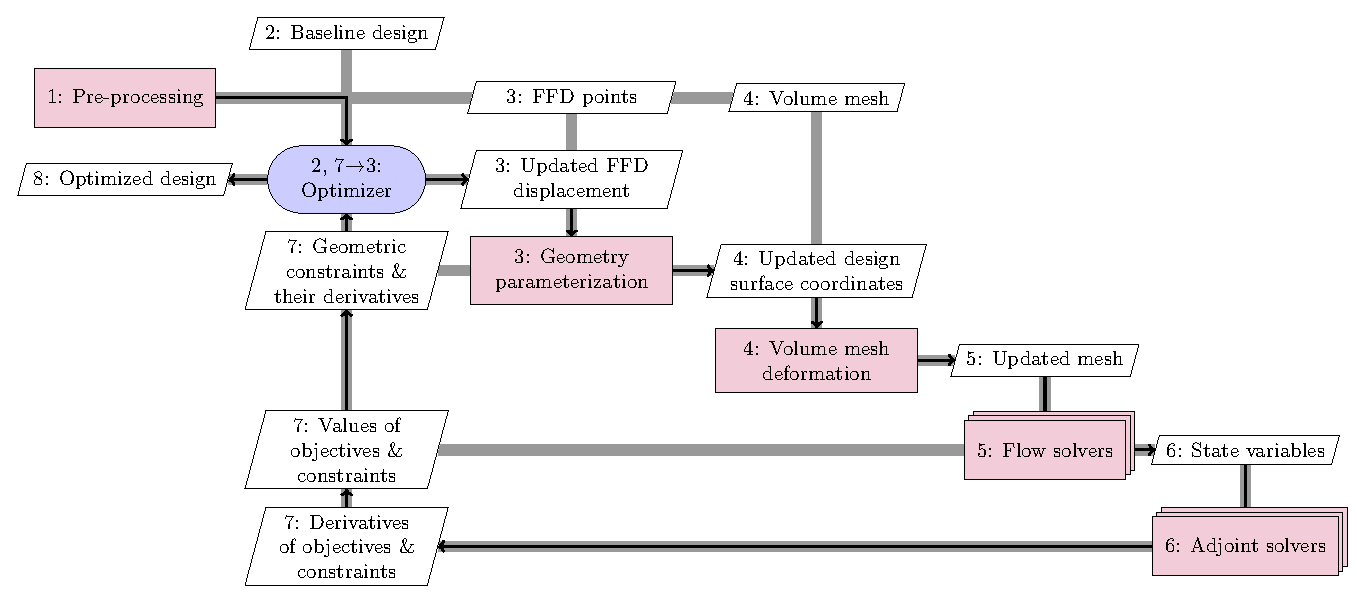
\includegraphics[width=\linewidth]{images/MACH-Aero-XDSM.pdf} 
    \caption{XDSM diagram for the MACH-Aero framework. The diagonal blocks are the modules (libraries) used in an optimization. The off-diagonal blocks are date transfer. All the modules are wrapped with Python.}
  \end{figure}
\end{frame}
%---------------------------------------------------------------%

%---------------------------------------------------------------%
\begin{frame}{Pre-processing module}
  \textbf{Goal}: Generate mesh and free-form deformation (FFD) control points

  Mesh needs to be in OpenFOAM format. Possible tools:
  \begin{itemize}
    \setlength\itemsep{1em}
    \item blockMesh and snappyHexMesh utilities from OpenFOAM.
    \item pyHyp (\url{https://github.com/mdolab/pyhyp}) from MACH-Aero.
    \item Commercial software such as ICEM-CFD, Pointwise.
  \end{itemize}

  FFD file needs to be in the \textbf{plot3D} format. Possible tools:
  \begin{itemize}
    \setlength\itemsep{1em}
    \item Python scripts such as genFFD.py.
    \item Commercial software that can generate structured meshes in the plot3D format, e.g., ICEM-CFD
  \end{itemize}
\end{frame}
%---------------------------------------------------------------%

%---------------------------------------------------------------%
\begin{frame}{Optimizer module}
  \textbf{Goal}: Receive function values and derivatives and update the design variables

  MACH-Aero uses pyOptSparse to set up optimization problems \url{https://github.com/mdolab/pyoptsparse} (Design variables, objective and constraint functions, and optimizers: SNOPT, SLSQP, IPOPT, etc.)
  \vspace{-0.15in}
  \begin{figure}
    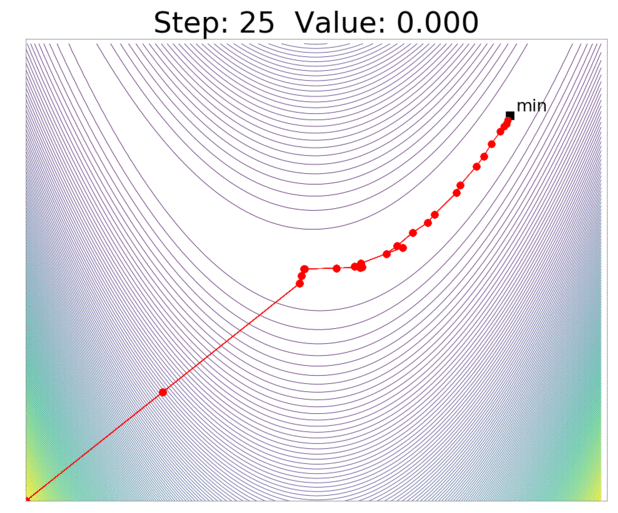
\includegraphics[width=0.5\linewidth]{images/rosenbrock.png}
    \caption{Optimization of the Rosenbrock function using gradient-based algorithms}
  \end{figure}
\end{frame}
%---------------------------------------------------------------%

%---------------------------------------------------------------%
\begin{frame}{Geometry parameterization module}
  \textbf{Goal}: Receive the updated design variables and change the design surface geometry or mesh.

  We use the pyGeo module to parameterize the geometry through the free-form deformation (FFD) approach (\url{https://github.com/mdolab/pygeo})
  \vspace{-0.15in}
  \begin{figure}
    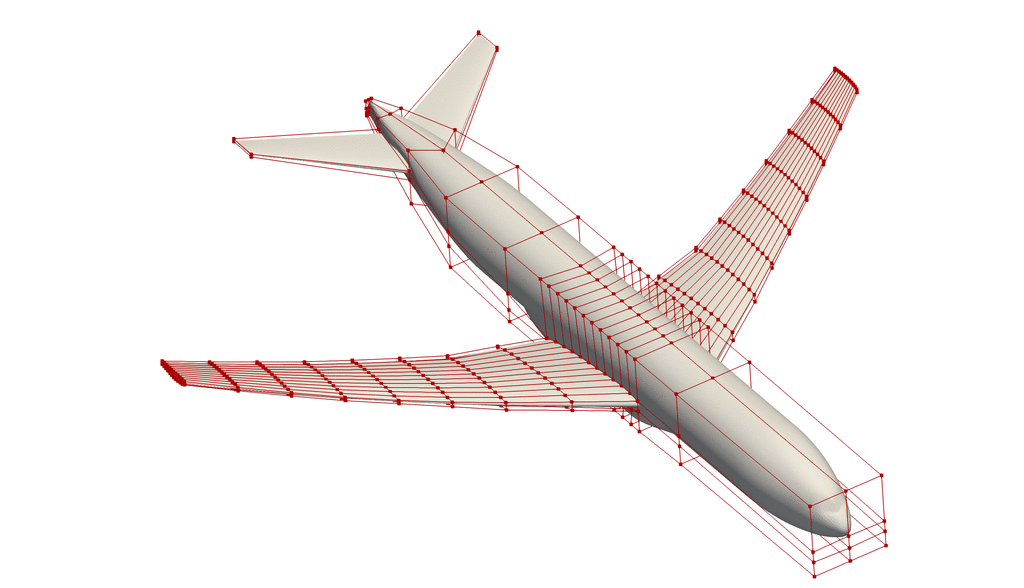
\includegraphics[width=0.85\linewidth]{images/DPW4_FFD.png}
    \caption{FFD control points (red) for an aircraft configuration}
  \end{figure}
\end{frame}
%---------------------------------------------------------------%


%---------------------------------------------------------------%
\begin{frame}{Volume mesh deformation module}
  \textbf{Goal}: Receive the design surface mesh and update the volume mesh coordinates

  We use the IDWarp module to deform the volume mesh through an inverse distance weighting approach. It works for both structured and unstructured meshes. (\url{https://github.com/mdolab/idwarp}). 
  \vspace{-0.1in}
  \begin{figure}
    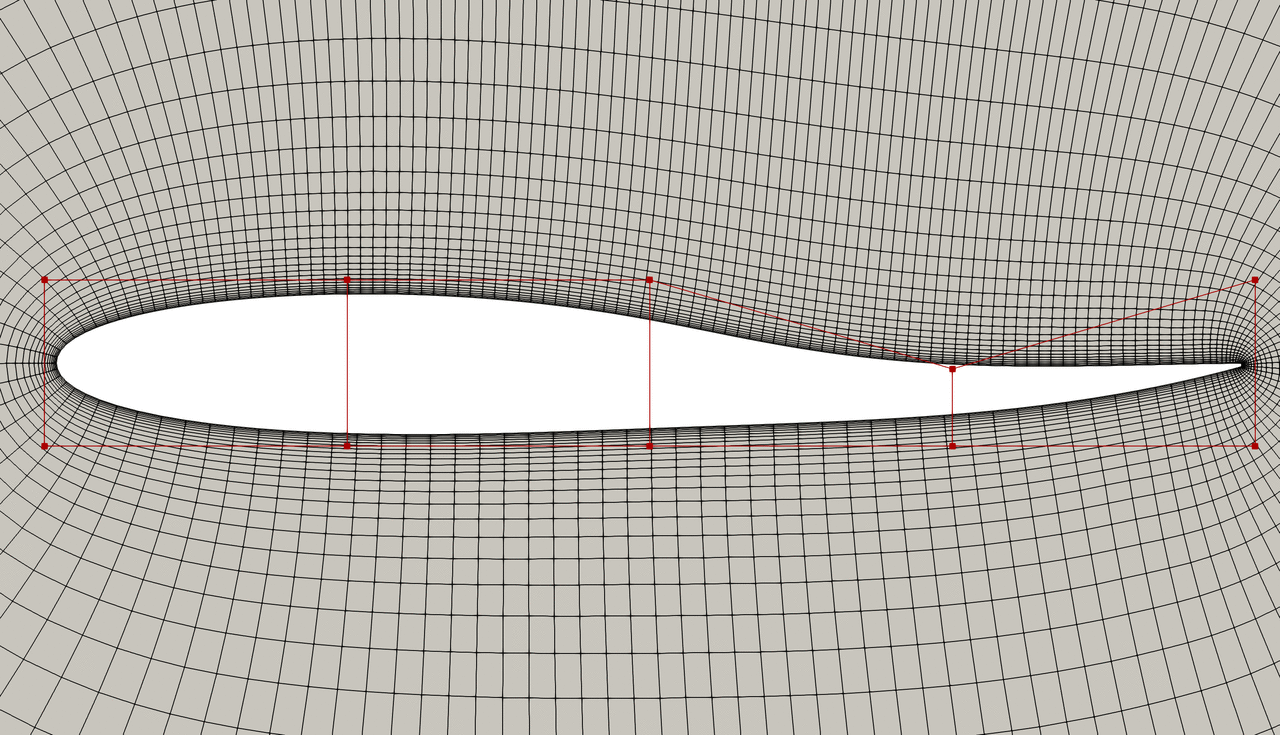
\includegraphics[width=0.8\linewidth]{images/NACA0012_Mesh_Deformation.png}
    \caption{Example of deformed mesh}
  \end{figure}
\end{frame}
%---------------------------------------------------------------%

%---------------------------------------------------------------%
\begin{frame}{Primal solution module}
  \textbf{Goal}: Receive the update volume mesh and compute the objective and constraint functions, as well as state variables (e.g., velocity and pressure). For fluid mechanics, it is also called flow simulation.

  We use Cython to compile OpenFOAM's solvers, e.g., simpleFoam, into C++ libraries and call them from Python. We do \textbf{NOT} use the OpenFOAM's built in binary solvers in optimization.
  \vspace{-0.1in}
  \begin{figure}
    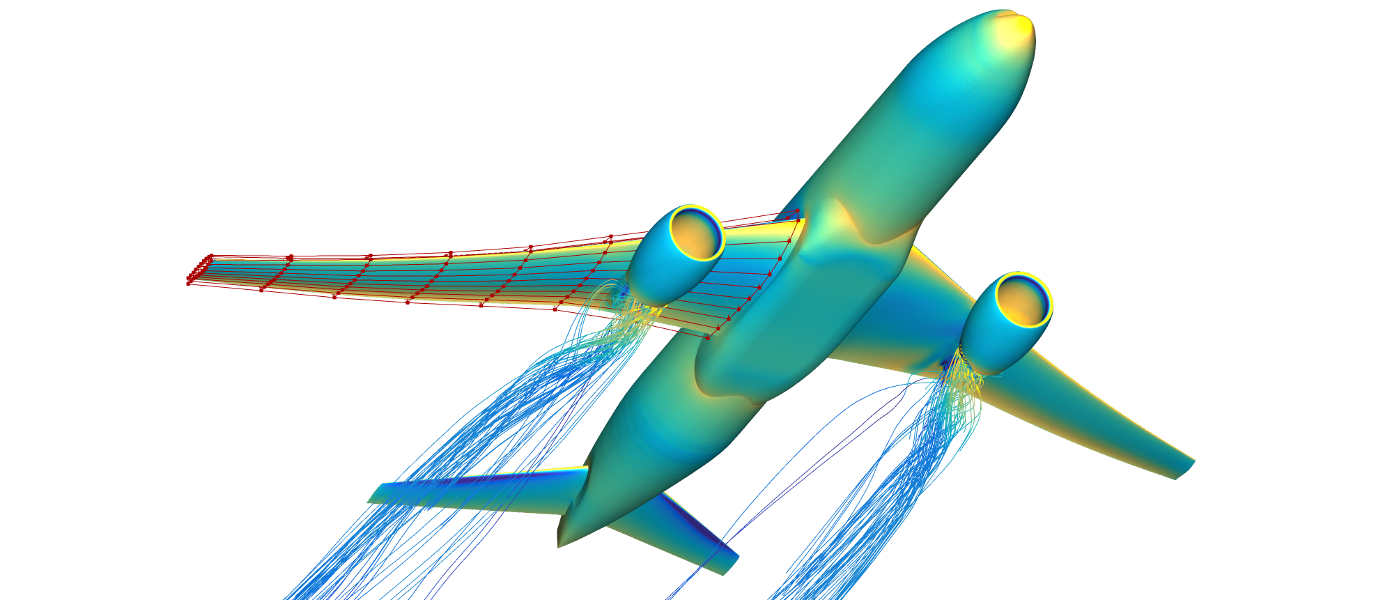
\includegraphics[width=\linewidth]{images/DPW6Flow.png}
    \caption{Aircraft aerodynamic analysis with OpenFOAM}
  \end{figure}
\end{frame}
%---------------------------------------------------------------%


%---------------------------------------------------------------%
\begin{frame}{Adjoint solution module}
  \textbf{Goal}: Receive the state variables and compute the total derivatives of objective functions with respect to all design variables

  We implemented efficient derivative computation in DAFoam using the Jacobian-free adjoint approach. The derivative is machine-precision accurate.
  \vspace{-0.1in}
  \begin{figure}
  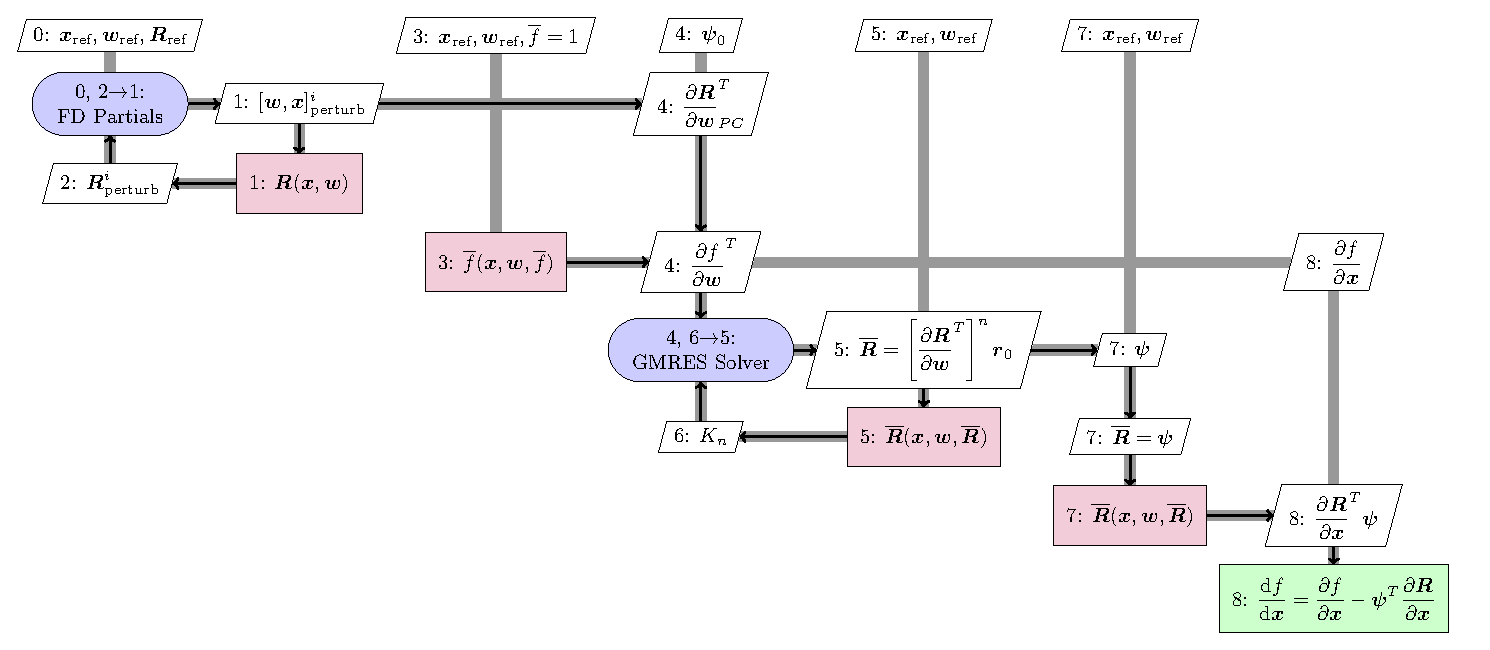
\includegraphics[width=\linewidth]{images/JacobianFreeDiagram.pdf}
  \caption{Jacobian-free adjoint diagram in DAFoam.}
  \end{figure}
\end{frame}
%---------------------------------------------------------------%


\section{Airfoil aerodynamic optimization}
\renewcommand{\arraystretch}{2}

%---------------------------------------------------------------%
\begin{frame}{}
  \center \Large Airfoil aerodynamic optimization
\end{frame}
%---------------------------------------------------------------%

%---------------------------------------------------------------%
\begin{frame}{Outline}
  \center \normalsize
  \begin{itemize}
    \setlength\itemsep{1em}
    \item How to use the DAFoam docker image
    \item How to run an optimization
    \item How to visualize the result
    \item How to read the optimization log file
    \item Details of configuration files
    \item How to change the configuration files for a new case
  \end{itemize}
\end{frame}
%---------------------------------------------------------------%

%---------------------------------------------------------------%
\begin{frame}{}
  \center \Large How to use the DAFoam docker image
\end{frame}
%---------------------------------------------------------------%


%---------------------------------------------------------------%
\begin{frame}[fragile]{Download DAFoam Docker image and examples}

  The easiest way to run DAFoam optimizations is to use the DAFoam Docker image

  First, install Docker following this website: \\ \vspace{0.1in} \small \url{https://dafoam.github.io/mydoc_get_started_download_docker.html} \normalsize

  Once done, verify the installation by running:
  \footnotesize
  \lstset{ language=bash }
  \begin{lstlisting}
  docker --version
  \end{lstlisting}
  \normalsize
     
  Then run this command to download the DAFoam Docker image: 

  \footnotesize
  \lstset{ language=bash }
  \begin{lstlisting}
  docker pull dafoam/opt-packages:v2.2.5
  \end{lstlisting}
  \normalsize
  
  Finally, download the workshop examples at: \\ \vspace{0.1in}
  \small \texttt{\url{https://github.com/dafoam/workshops}}

\end{frame}
%---------------------------------------------------------------%

%---------------------------------------------------------------%
\begin{frame}[fragile]{How to start a Docker container}

  If you use Linux or MacOS, open a terminal and use the \texttt{cd} command to go this folder on your local computer. If you put the workshops folder in the \$HOME directory, the command may look like:

  \footnotesize
  \begin{lstlisting}
  cd $HOME/workshops/2021_Summer/examples/naca0012/incompressible
  \end{lstlisting}
  \normalsize
  
  Then, run this command to start a Docker container:

  \footnotesize
  \begin{lstlisting}
  docker run -it --rm -u dafoamuser --mount \
  "type=bind,src=$(pwd),target=/home/dafoamuser/mount" \ 
  -w /home/dafoamuser/mount dafoam/opt-packages:v2.2.5 bash
  \end{lstlisting}
  \normalsize

  If you use Windows, open the Prompt Command terminal, use the \texttt{cd} command to go to the above folder, and run this command: \\ \vspace{0.1in}

  \footnotesize
  \begin{lstlisting}
  docker run -it --rm -u dafoamuser --mount \
  "type=bind,src=%cd%,target=/home/dafoamuser/mount" \
  -w /home/dafoamuser/mount dafoam/opt-packages:v2.2.5 bash
  \end{lstlisting}
  \normalsize

  Once in a Docker container, you should see something like:
  \footnotesize
  \lstset{ language=bash }
  \begin{lstlisting}
  dafoamuser@cddb89839078:~/mount$ 
  \end{lstlisting}
  \normalsize

\end{frame}
%---------------------------------------------------------------%

%---------------------------------------------------------------%
\begin{frame}[fragile]{More information about the Docker container}

  What does the above command do? \vspace{-0.1in}
  \begin{itemize}
    \setlength\itemsep{0.2em}
     \item Start a Docker container (a light-weight virtual machine)
     \item Mount (link) your computer's current directory to the container’s /home/dafoamuser/mount directory
     \item Login the container as dafoamuser and go to the mounted dir
     \item Set the relevant DAFoam environmental variables. 
  \end{itemize}
  A few notes:  \vspace{-0.1in}
  \begin{itemize}
    \setlength\itemsep{0.2em}
    \item Treat the Docker container as disposable, i.e., start one container for one optimization run. If the optimization is running and you want to kill it, press \texttt{ctrl+c} or \texttt{ctrl+\textbackslash} to kill the job, then run \texttt{exit} to quit the container
    \item Do not store simulation results in the container because they will be deleted after you exit. Run simulations on the mounted space \texttt{/home/dafoamuser/mount} instead
    \item dafoamuser has the sudo privilege and its password is: dafoamuser
  \end{itemize}

\end{frame}
%---------------------------------------------------------------%

%---------------------------------------------------------------%
\begin{frame}{}
  \center \Large How to run an optimization
\end{frame}
%---------------------------------------------------------------%

\begin{frame}{How to run an optimization (1/3)}
  \begin{table}
    \renewcommand{\arraystretch}{1.5}
    \small
    \centering
    \caption{\small Summary of the naca0012/incompressible case.}
    \label{tab:implemented_models}
    \begin{tabular}{llllllllllll}
    \hline
    Optimizer   & IPOPT \\
    Flow and adjoint solvers  & DASimpleFoam  \\
    Geometry  & NACA0012 \\
    Mesh  & 4\,032 cells\\
    Objective function  & $C_d$ \\
    Design variables & 20 FFDs and $\alpha$ \\
    Constraint & $C_l=0.5$, thickness, volume, TE/LE \\
    $U_\infty$  & 10 m/s \\
    $Re$  & 6.7$\times10^5$\\
    Turbulence Model  & Spalart--Allmaras\\
     \hline
    \end{tabular}
  \end{table}
\end{frame}

%---------------------------------------------------------------%
\begin{frame}[fragile]{How to run an optimization (2/3)}

  Once in a Docker container, you should see something like:
  \footnotesize
  \lstset{ language=bash }
  \begin{lstlisting}
  dafoamuser@cddb89839078:~/mount$ 
  \end{lstlisting}
  \normalsize
  
  Run this command to double check if you are in the correct directory:
  \footnotesize
  \lstset{ language=bash }
  \begin{lstlisting}
  ls
  \end{lstlisting}
  \normalsize

  After running the above command, you should see something like:
  \footnotesize
  \lstset{ language=bash }
  \begin{lstlisting}
  0.orig  Allclean.sh  FFD  constant  genAirFoilMesh.py  paraview.foam 
  preProcessing.sh  profiles  runScript.py  system
  \end{lstlisting}
  \normalsize

\end{frame}
%---------------------------------------------------------------%

%---------------------------------------------------------------%
\begin{frame}[fragile]{How to run an optimization (2/3)}

  Once in a Docker container, you should see something like:
  \footnotesize
  \lstset{ language=bash }
  \begin{lstlisting}
  dafoamuser@cddb89839078:~/mount$ 
  \end{lstlisting}
  \normalsize
  
  Run this command to double check if you are in the correct directory:
  \footnotesize
  \lstset{ language=bash }
  \begin{lstlisting}
  ls
  \end{lstlisting}
  \normalsize

  After running the above command, you should see something like:
  \footnotesize
  \lstset{ language=bash }
  \begin{lstlisting}
  0.orig  Allclean.sh  FFD  constant  genAirFoilMesh.py  paraview.foam 
  preProcessing.sh  profiles  runScript.py  system
  \end{lstlisting}
  \normalsize

\end{frame}
%---------------------------------------------------------------%


%---------------------------------------------------------------%
\begin{frame}[fragile]{How to run an optimization (3/3)}

  Now you should be in the right directory. There are two main steps to run a case.

  First, run this command for pre-processing (mesh generation):
  \footnotesize
  \lstset{ language=bash }
  \begin{lstlisting}
  ./preProcessing.sh
  \end{lstlisting}
  \normalsize

  Then, use this command to run the flow simulation: 
  \footnotesize
  \lstset{ language=bash }
  \begin{lstlisting}
  python runScript.py | tee 2>&1 logOpt.txt
  \end{lstlisting}
  \normalsize

  The optimization log will be printed to the screen and saved to \texttt{logOpt.txt}. In addition, the optimizer will write a separate log to the disk. For the IPOPT optimizer we use in this tutorial, it is \texttt{opt\_IPOPT.txt}.

  The optimization converged in 17 steps and took about 10 minutes.

\end{frame}
%---------------------------------------------------------------%

%---------------------------------------------------------------%
\begin{frame}{}
  \center \Large How to visualize the results
\end{frame}
%---------------------------------------------------------------%

%---------------------------------------------------------------%
\begin{frame}{How to visualize the results (1/7)}

  We use Paraview; an open-source post-processing tool to visualize the optimization results.

  \begin{itemize}
    \setlength\itemsep{1em}
    \item Download Paraview at \url{https://www.paraview.org/download/}. 
    \item For MacOS, download \texttt{ParaView-5.8.1-MPI-OSX10.12-Python2.7-64bit.dmg} and install the .dmg package
    \item For Ubuntu, download \texttt{ParaView-5.8.1-MPI-Linux-Python2.7-64bit.tar.gz}, extract the tarball, and run the paraview executive in the ParaView-5.8.1-MPI-Linux-Python2.7-64bit/bin folder
    \item For Windows, download \texttt{ParaView-5.8.1-Windows-Python3.7-msvc2015-64bit.zip}, extract the zip and run the paraview executive in the ParaView-5.8.1-Windows-Python3.7-msvc2015-64bit/bin folder
 \end{itemize}
\end{frame}
%---------------------------------------------------------------%

%---------------------------------------------------------------%
\begin{frame}{How to visualize the results (2/7)}
  In Paraview, click \texttt{File->Open}. In the pop up window, select \texttt{paraview.foam} in the \texttt{naca0012/incompressible} folder, and click \texttt{OK}.
  
  \begin{figure}
    \centering
    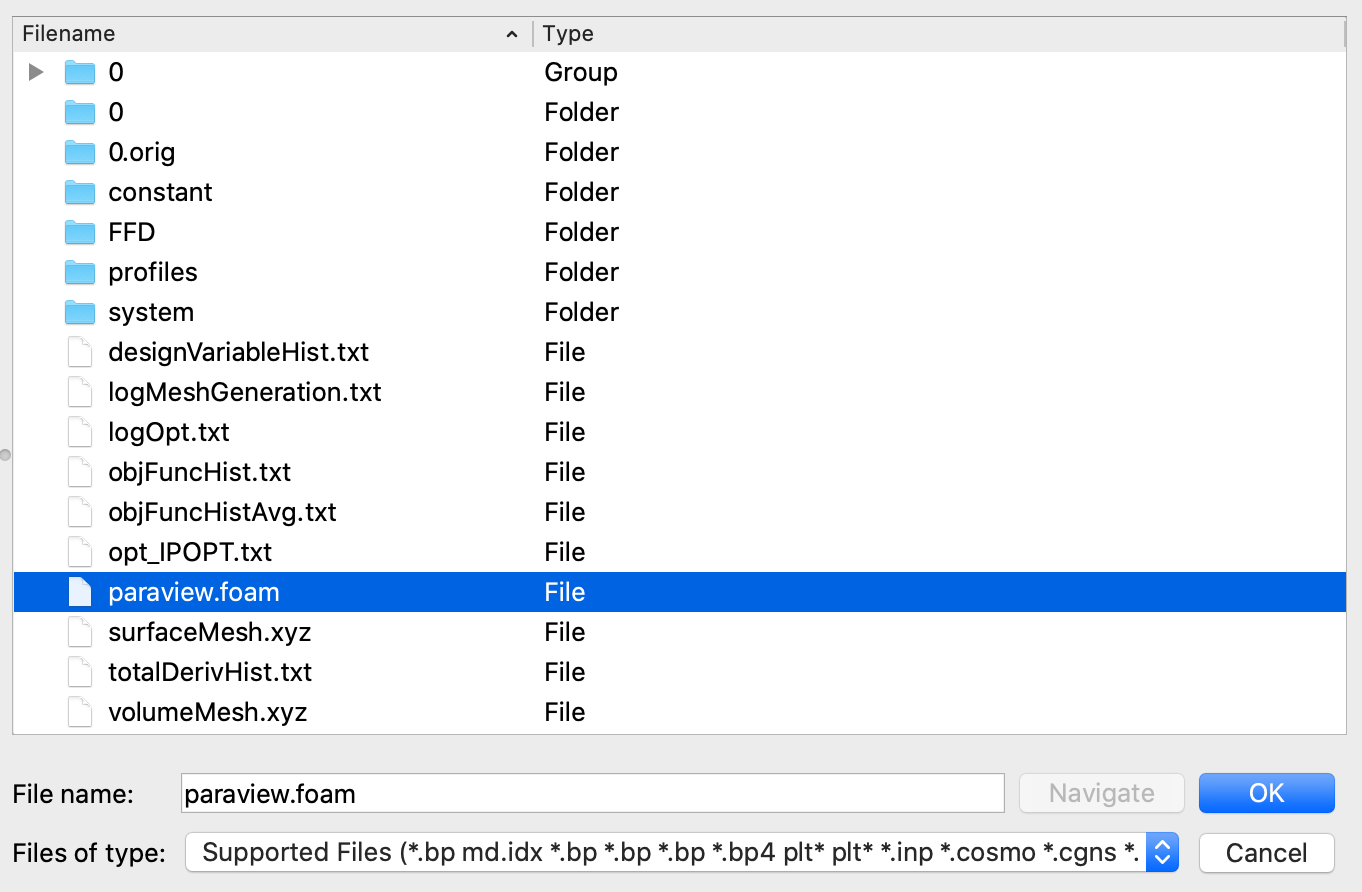
\includegraphics[width=4.0in]{images/paraview_open.png} 
  \end{figure}
\end{frame}
%---------------------------------------------------------------%

%---------------------------------------------------------------%
\begin{frame}{How to visualize the results (3/7)}
  Then, on the left properties window, hit \texttt{Apply}.
  
  \begin{figure}
    \centering
    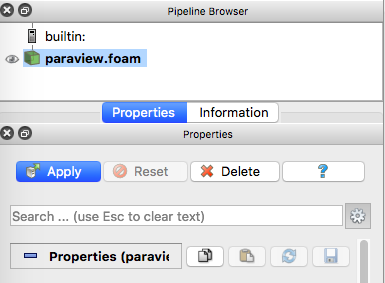
\includegraphics[width=3.in]{images/paraview_open_apply.png}
  \end{figure}
\end{frame}
%---------------------------------------------------------------%

%---------------------------------------------------------------%
\begin{frame}{How to visualize the results (4/7)}
  Finally, you can see the simulation results for the NACA0012 airfoil on the right layout window
  
  \begin{figure}
    \centering
    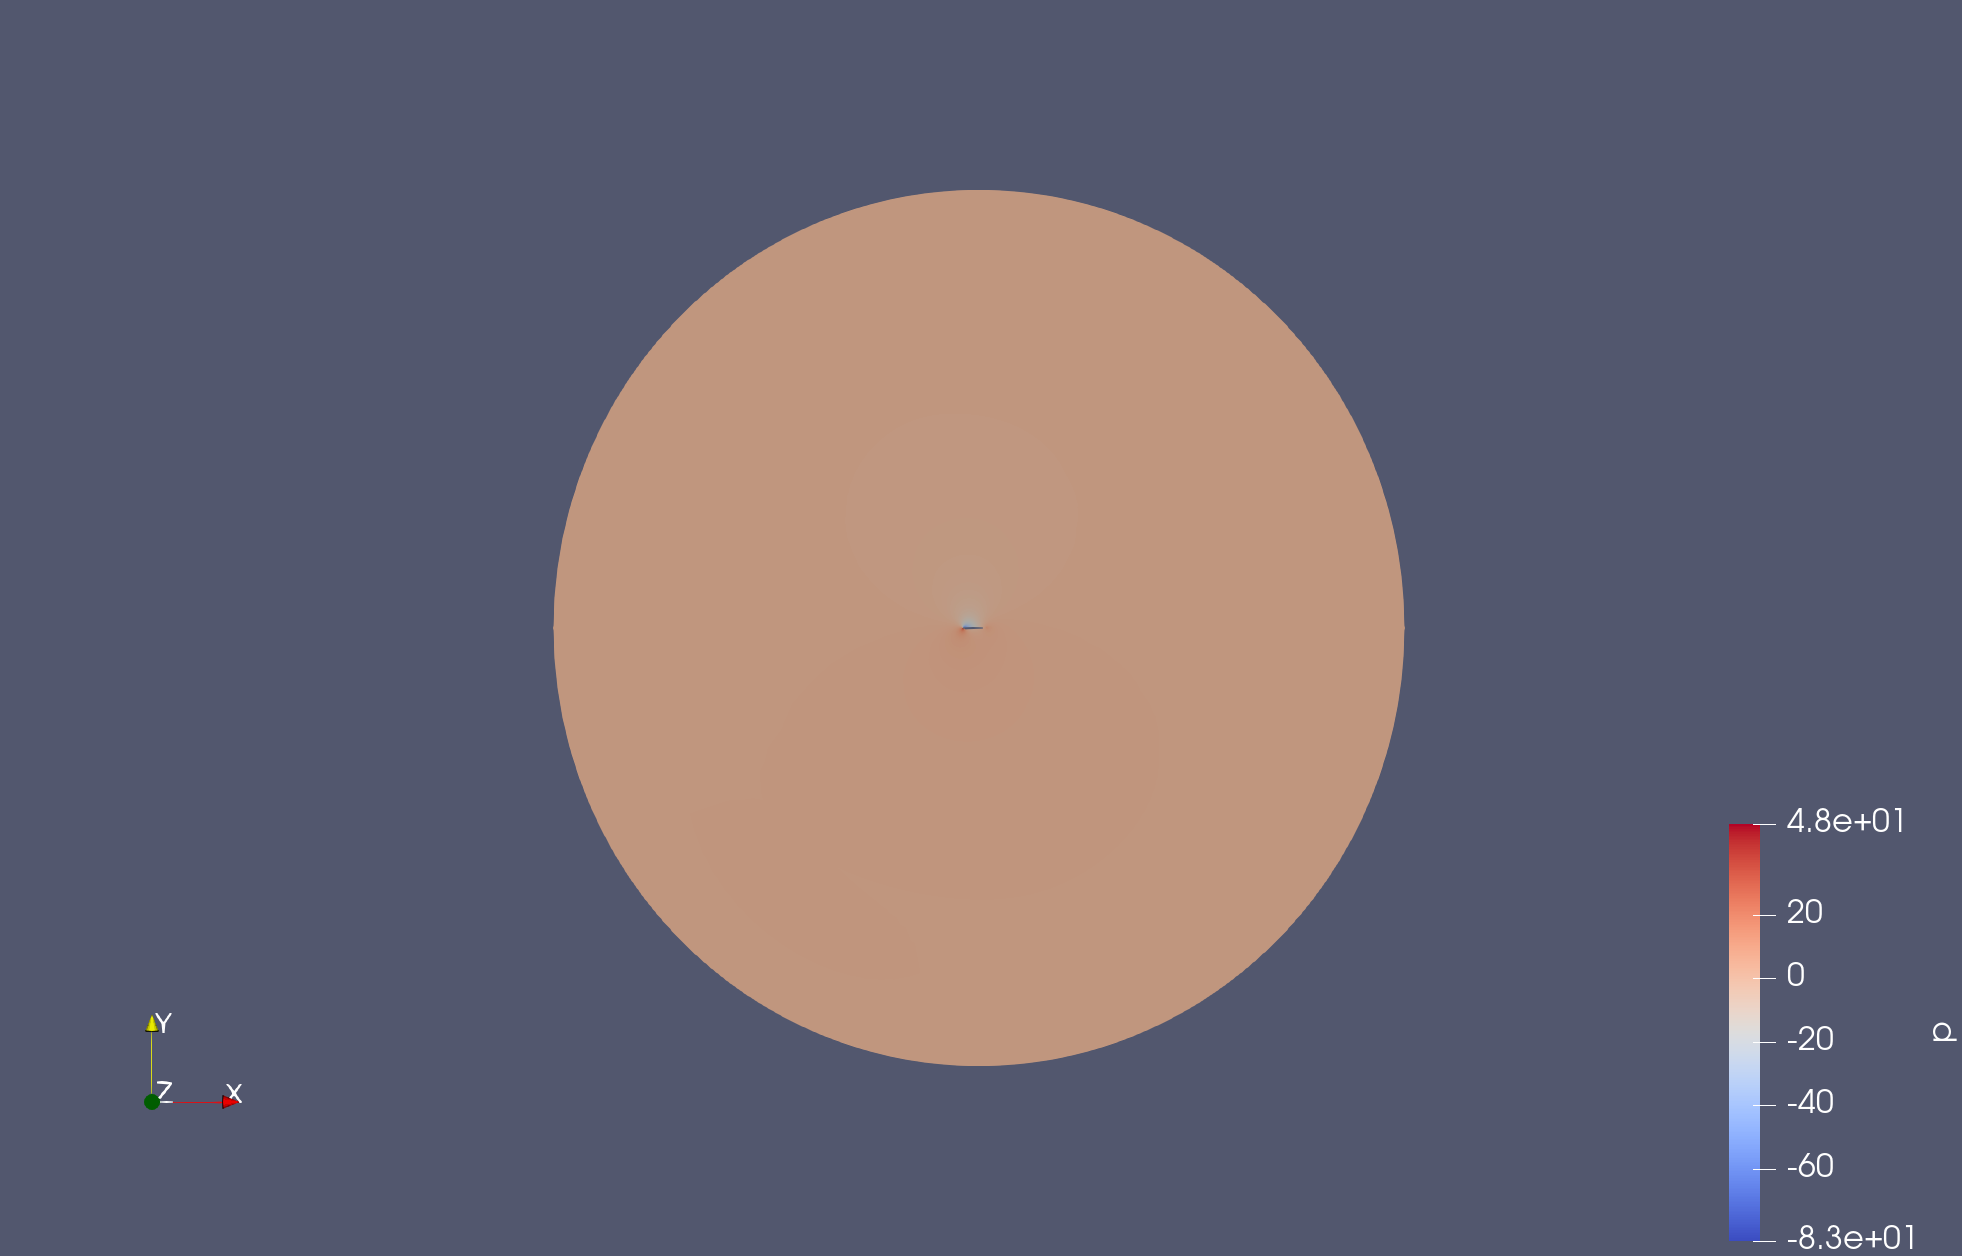
\includegraphics[width=3.8in]{images/paraview_initial_view.png}
  \end{figure}
\end{frame}
%---------------------------------------------------------------%


%---------------------------------------------------------------%
\begin{frame}{How to visualize the results (5/7)}
  You can scroll your mouse wheel to zoom-in and zoom-out, and hold your middle wheel, you can pan the view.

  We also recommend enable the \texttt{Camera Parallel Projection} option by first clicking this icon on the left properties bar
  \begin{figure}
    \centering
    
\includegraphics[width=0.3in]{images/paraview_gear.png}
  \end{figure}

  Then, scroll down and check \texttt{Camera Parallel Projection}
  \begin{figure}
    \centering
    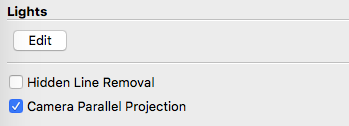
\includegraphics[width=3.in]{images/paraview_parallel_camera.png}
  \end{figure}
\end{frame}
%---------------------------------------------------------------%

%---------------------------------------------------------------%
\begin{frame}{How to visualize the results (6/7)}
  Now, you can zoom-in to view the detailed pressure field around the airfoil (scroll your mouse wheel).
  \begin{figure}
    \centering
    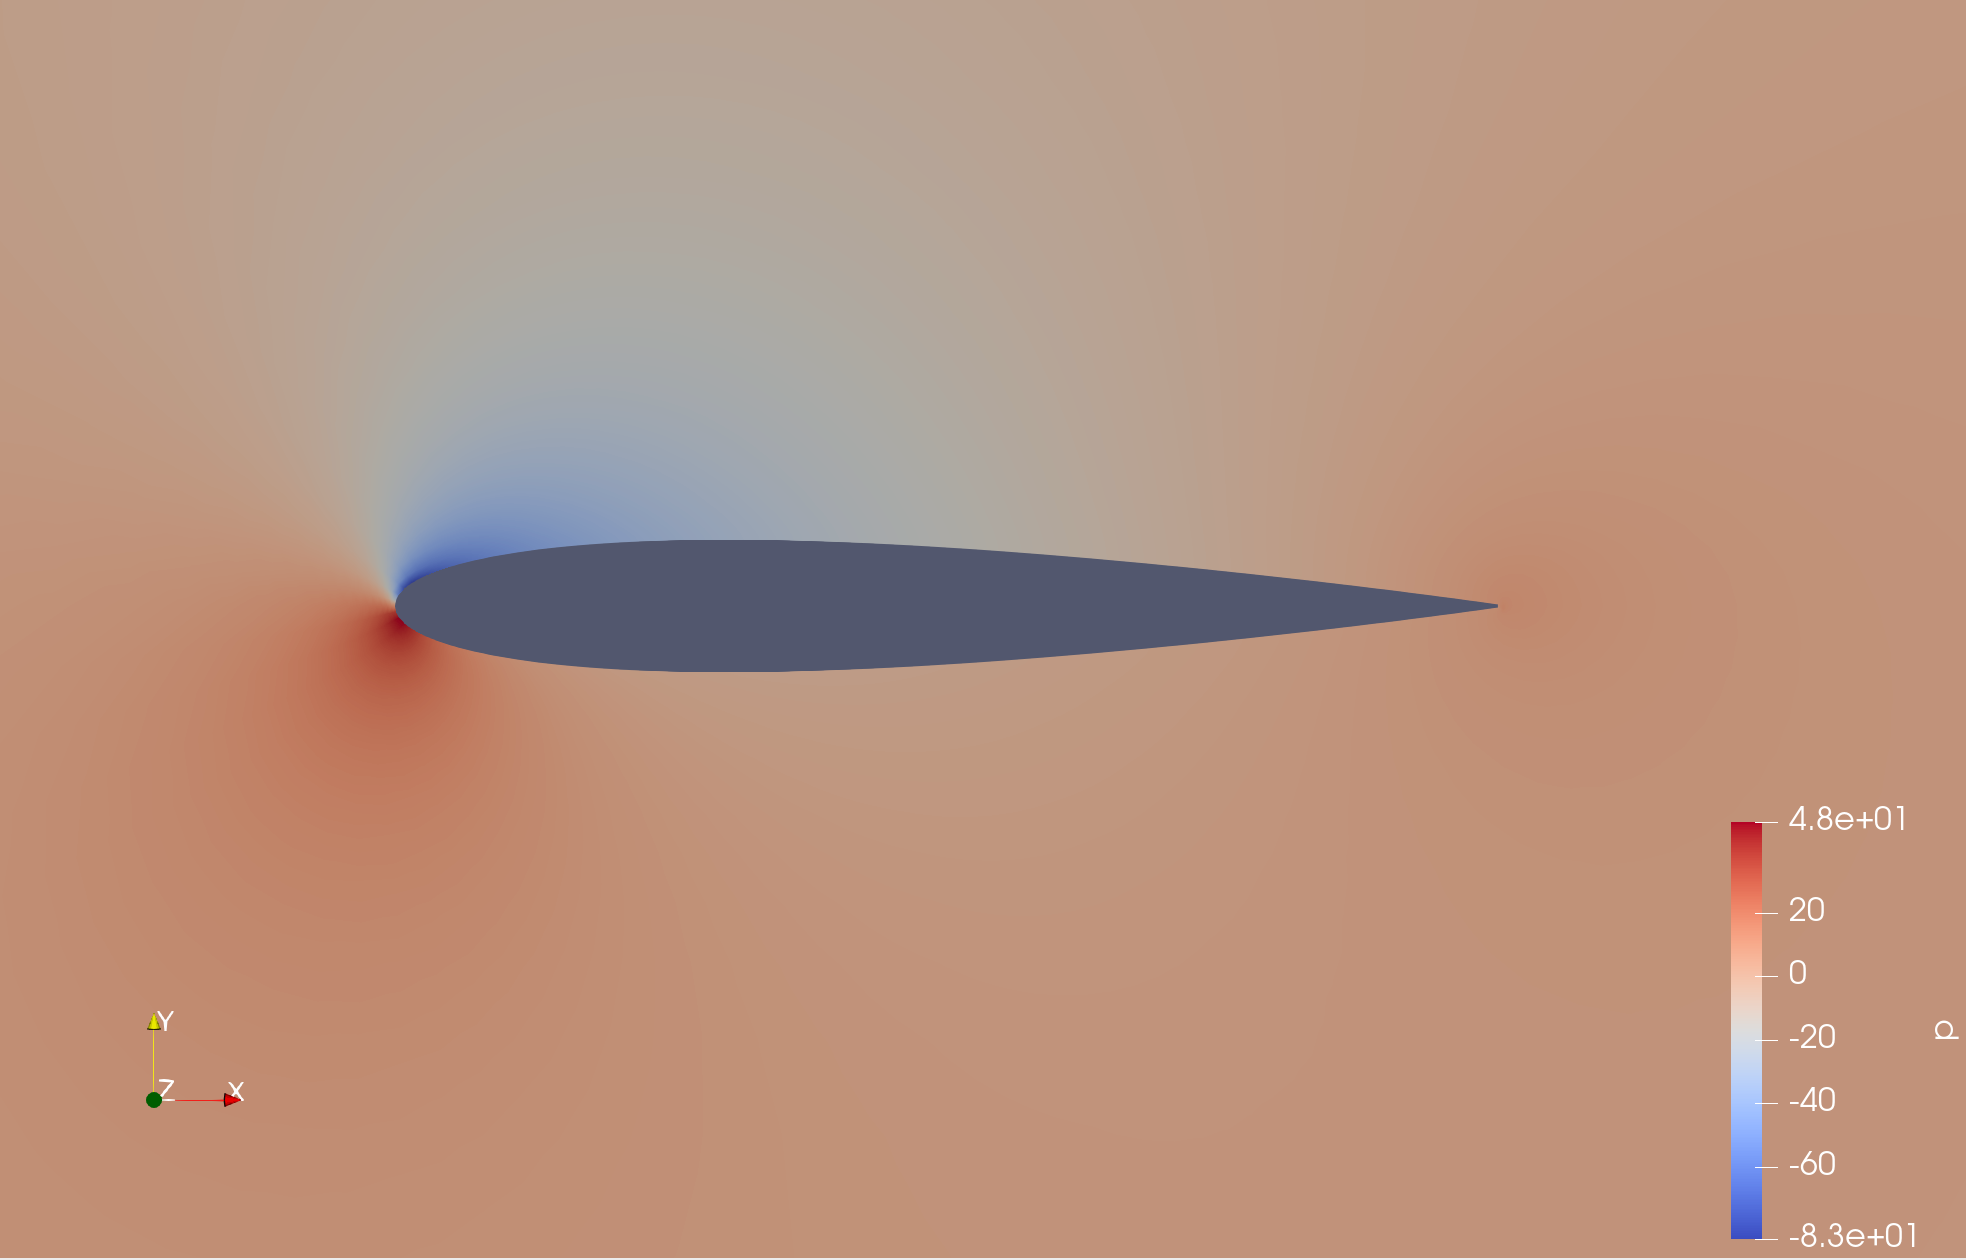
\includegraphics[width=3.5in]{images/paraview_pressure.png}
  \end{figure}

\end{frame}
%---------------------------------------------------------------%

%---------------------------------------------------------------%
\begin{frame}{How to visualize the results (7/7)}
  Now you can hit the \texttt{play} button on the top bar to visualize the evolution of pressure and shape during the optimization.
  \begin{figure}
    \centering
    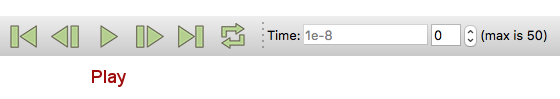
\includegraphics[width=3in]{images/paraview_play.png}
  \end{figure}
  If you want to look at another variable, change the range of the variable, or change the surface representation (e.g., visualize the mesh), check the top bar as shown below.
  \begin{figure}
    \centering
    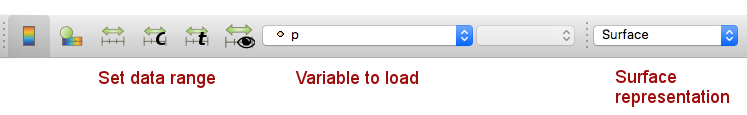
\includegraphics[width=4in]{images/paraview_var_scale_surface.png}
  \end{figure}

\end{frame}
%---------------------------------------------------------------%

%---------------------------------------------------------------%
\begin{frame}{}
  \center \Large How to read optimization log files
\end{frame}
%---------------------------------------------------------------%

%---------------------------------------------------------------%
\begin{frame}[fragile]{How to read \texttt{opt\_IPOPT.txt}}

\texttt{opt\_IPOPT.txt} is the very first file we need to check during or after the optimization. We want to look at the objective, feasibility (inf\_pr) and optimality (inf\_du).

A successful optimization should reduce the objective function values, and the feasibility and optimality should drop below the prescribed tolerance (1e-6 for this tutorial).

\scriptsize
\begin{lstlisting}
iter    objective    inf_pr   inf_du lg(mu)  ||d||  lg(rg) alpha_du alpha_pr  ls
0  2.0820238e-02 1.61e-07 1.43e-02   0.0 0.00e+00    -  0.00e+00 0.00e+00   0
1  2.0522813e-02 3.29e-04 6.87e-02  -5.9 7.45e-03    -  9.54e-01 1.00e+00h  1
2  1.9625311e-02 2.41e-03 2.67e-01  -7.3 2.14e-02    -  9.69e-01 1.00e+00h  1
3  1.9219882e-02 1.06e-03 4.45e-03  -4.4 3.51e-02    -  9.89e-01 1.00e+00h  1
4  1.9054431e-02 1.56e-04 2.14e-03  -4.9 9.26e-02    -  1.00e+00 1.00e+00h  1
5  1.8964830e-02 5.90e-05 1.25e-03  -5.8 5.98e-02    -  1.00e+00 1.00e+00h  1
.........
13  1.7376934e-02 2.93e-05 2.45e-04  -6.7 2.93e-02    -  1.00e+00 1.00e+00h  1
14  1.7376357e-02 6.27e-07 3.25e-06  -8.4 7.27e-03    -  1.00e+00 1.00e+00h  1
15  1.7376337e-02 1.09e-07 1.56e-06 -10.2 3.16e-03    -  1.00e+00 1.00e+00h  1
16  1.7376337e-02 6.04e-10 1.03e-06 -11.0 1.07e-04    -  1.00e+00 1.00e+00h  1
17  1.7376337e-02 2.50e-09 5.61e-07 -11.0 6.01e-04    -  1.00e+00 1.00e+00h  1
\end{lstlisting}

\end{frame}
%---------------------------------------------------------------%

%---------------------------------------------------------------%
\begin{frame}{Flow and adjoint equations}

In flow solution, the steady-state incompressible Navier-Stokes equations are solved using the finite-volume mesh with the SIMPLE algorithm:

$\nabla \cdot \boldsymbol{U} = 0$

$(\boldsymbol{U} \cdot \nabla) \boldsymbol{U}  +  \nabla p -  \nabla \cdot \nu_{eff} (\nabla \boldsymbol{U} +\nabla \boldsymbol{U}^T) = 0$ 

\vspace{+0.1in}

In adjoint solution, the adjoint equation is solved using a Jacobian free method to get the adjoint vector $\psi$

$[\dfrac{\partial \boldsymbol{R}}{\partial \boldsymbol{W}}]^T \psi = \dfrac{\partial f}{\partial \boldsymbol{W}}$

Then, the adjoint vector is used to compute the total derivative $\dif f/\dif \boldsymbol{x}$.

$\dfrac{\dif f}{\dif \boldsymbol{x}}= \dfrac{\partial f}{\partial \boldsymbol{x}} - [\dfrac{\partial \boldsymbol{R}}{\partial \boldsymbol{x}}]^T \psi$

\end{frame}
%---------------------------------------------------------------%
  


%---------------------------------------------------------------%
\begin{frame}[fragile]{How to read \texttt{logOpt.txt} (1/8)}

  Basic information.
  \scriptsize
  \lstset{ language=c++ }
  \begin{lstlisting}
  -----------------------------------------------------------------------------
  |                                  DAFoam v2.2.5                                     |
  -----------------------------------------------------------------------------
  Selecting RAS turbulence model SpalartAllmaras // Turbulence model
  ...
  Global Cells: 4032  // Mesh cells
  DAFoam option dictionary: // All DAFoam options 
  {
    solverName      DASimpleFoam;
    primalMinResTol 1e-08;
    ...
  }
  +---------------------------------------+
  |     All IDWarp Options:               |
  +---------------------------------------+
   {'LdefFact': 1.0,  // All IDWarp options
    'aExp': 3.0,
    'alpha': 0.25,
    ....
  #------------------------------#
  Total Volume Nodes :     17640 
  #------------------------------#
  {'all': [3, 4],  // Design surface information
   'allsurfaces': [0, 1, 2, 3, 4],
   'designsurfaces': [3, 4],
  \end{lstlisting}

\end{frame}
%---------------------------------------------------------------%

%---------------------------------------------------------------%
\begin{frame}[fragile]{How to read \texttt{logOpt.txt} (2/8)}

  Before running the optimization, it automatically finds the angle of attack to match the target CL (0.5). This is also called solveCL.
  \scriptsize
  \lstset{ language=c++ }
  \begin{lstlisting}
  +--------------------------------------------------------------------------+
  |                 Running SolveCL to find alpha that matches target CL           |
  +--------------------------------------------------------------------------+
  eps: 0.01  tol: 0.0001  maxit: 10 // eps: solveCL finite-difference step size
  +--------------------------------------------------------------------------+
  |                     Evaluating Objective Functions 000                         |
  +--------------------------------------------------------------------------+
  Design Variables: 
  {'alpha': array([5.+0.j]), ... }
  ...
  Setting U = (9.961947 0.87155743 0) at inout // setting U field based on alpha
  ...
  Time = 400
  U Initial residual: (1.5179219e-08 1.1995847e-08 1.5597788e-08)
  U   Final residual: (1.1435775e-09 9.1588646e-10 1.3379879e-09)
  ...
  yPlus min: 14.568982 max: 100.52633 mean: 60.130968 // flow solution prints y+
  CD-part1-force: 0.020495205 // CD and CL at Time = 400
  CL-part1-force: 0.48750507
  ExecutionTime = 8.69 s  ClockTime = 10 s
  Time = 425 // flow converged in 425 steps
  Minimal residual 9.8369143e-09 satisfied the prescribed tolerance 1e-08
  alpha: 5.000000, CL: 0.487505 // first solved alpha and CL
  ... // repeat the solveCL
  alpha: 5.139185, CL: 0.500000 // final alpha and CL
  Completed! alpha = 5.139185
  \end{lstlisting}

\end{frame}
%---------------------------------------------------------------%


%---------------------------------------------------------------%
\begin{frame}[fragile]{How to read \texttt{logOpt.txt} (3/8)}

  Once solveCL is done, the optimization starts. It first prints the initial design variables, constraints, bounds, etc.
  \scriptsize
  \begin{lstlisting}
  Optimization Problem -- opt
  ================================================================================
  Objective Function: aeroFuncs
  Objectives
     Index  Name            Value          Optimum
         0  CD     0.E+00     0.E+00
  Variables (c - continuous, i - integer, d - discrete) // design variables
     Index  Name        Type      Lower Bound            Value      Upper Bound     Status
         0  alpha_0        c     0.E+00     5.139185E+00     1.E+01    
         1  shapey_0       c    -1.E-01     0.E+00     1.E-01           
         2  shapey_1       c    -1.E-01     0.E+00     1.E-01           
         3  shapey_2       c    -1.E-01     0.E+00     1.E-01                       
         ....
  Constraints (i - inequality, e - equality)  // constraints
  Index  Name                          Type    Lower     Value    Upper   Status  Pi(N/A)
  0  DVCon1_volume_constraint_0           i   1.E+00    0.E+00    3.E+00    L    9.E+100
  1  DVCon1_thickness_constraints_0       i   8.E-01    0.E+00    3.E+00    L    9.E+100
  2  DVCon1_thickness_constraints_0       i   8.E-01    0.E+00    3.E+00    L    9.E+100
  3  DVCon1_thickness_constraints_0       i   8.E-01    0.E+00    3.E+00    L    9.E+100    
      ....  
  \end{lstlisting}

\end{frame}
%---------------------------------------------------------------%

%---------------------------------------------------------------%
\begin{frame}[fragile]{How to read \texttt{logOpt.txt} (4/8)}

  Then, the coloring is computed. The coloring information will be used to compute the Jacobian matrices, e.g., dRdWTPC.
  \scriptsize
  \begin{lstlisting}
  +--------------------------------------------------------------------------+
  |                          Running Coloring Solver                               |
  +--------------------------------------------------------------------------+
  ...
  Calculating dRdW Coloring..
  number of uncolored: 36223 1
  ColorSweep: 100   8 s
  number of uncolored: 23511 1
  ColorSweep: 200   10 s
  number of uncolored: 11178 1
  ColorSweep: 300   12 s
  number of uncolored: 544 1
  ColorSweep: 324   13 s
  ...
  Calculating dFdW CD-part1 Coloring...
  ...
  \end{lstlisting}

\end{frame}
%---------------------------------------------------------------%

%---------------------------------------------------------------%
\begin{frame}[fragile]{How to read \texttt{logOpt.txt} (5/8)}

  It first solves the flow and computes the initial objective function.
  \scriptsize
  \begin{lstlisting}
  +--------------------------------------------------------------------------+
  |                     Evaluating Objective Functions 005                         |
  +--------------------------------------------------------------------------+
  Design Variables: 
  OrderedDict([('alpha', array([5.139184882352932])), ('shapey', array([0., ... 0.]))]) // all design variable values for this flow solution.
  ...
  // Check mesh quality before actually run the flow solution. If checkMesh fails, the flow solution will not run.
  Checking mesh quality for time = 0 
  Overall domain bounding box (-17.36956 -18.580929 0) (18.72809 18.580929 0.1)
  Mesh has 3 geometric (non-empty/wedge) directions 3{1}
  Mesh has 3 solution (non-empty) directions 3{1}
  Boundary openness (-4.6536375e-19 -3.9490374e-19 -5.6880426e-16) OK.
  Max cell openness = 2.4445483e-16 OK.
  Max aspect ratio = 97.871471 OK.
  Minimum face area = 2.2541308e-06. Maximum face area = 4.2248202.  Face area magnitudes OK.
  Min volume = 2.2541308e-07. Max volume = 0.42248202.  Total volume = 105.2804.  Cell volumes OK.
  Mesh non-orthogonality Max: 22.749125 average: 2.5479332
  Non-orthogonality check OK.
  Face pyramids OK.
  Max skewness = 1.4324517 OK.
  Coupled point location match (average 0) OK.
  Mesh OK. // checkMesh passes
  \end{lstlisting}

\end{frame}
%---------------------------------------------------------------%

%---------------------------------------------------------------%
\begin{frame}[fragile]{How to read \texttt{logOpt.txt} (6/8)}

  After the flow solution converges, it will print the objective and constraint function values.
  \scriptsize
  \begin{lstlisting}
  Time = 200
  U Initial residual: (8.0489602e-08 6.5681323e-08 1.9305741e-07) // U residual
  U   Final residual: (6.1866068e-09 4.979837e-09 1.6009007e-08)
  p Initial residual: 2.1616161e-07 // p residual
  p   Final residual: 1.4795847e-08
  Time step continuity errors : sum local = 3.8277947e-10
                                   global = -1.6582597e-11
                               cumulative = 0.00015887025
  nuTilda Initial residual: 2.2029223e-09 // turbulence variable residual
            Final residual: 2.1250661e-10
  Bounding nuTilda>1e-16
  yPlus min: 14.224415 max: 101.14689 mean: 59.937027 // y+
  CD-part1-force: 0.020820085 // drag coefficient
  CL-part1-force: 0.50000308  // lift coefficient
  ExecutionTime = 51.83 s  ClockTime = 58 s
  Time = 286
  Minimal residual 9.8182915e-09 satisfied the prescribed tolerance 1e-08
  // Print the converged objective and constraint functions for this solution
  Objective Functions: 
  {'DVCon1_volume_constraint_0': 1., 'DVCon1_thickness_constraints_0': array([1., ... 1.]), 'CD': 0.020820238430313175, 'CL': 0.5000001610403806, 'fail': False}
  Flow Runtime: 6.38911
  \end{lstlisting}

\end{frame}
%---------------------------------------------------------------%

%---------------------------------------------------------------%
\begin{frame}[fragile]{How to read \texttt{logOpt.txt} (7/8)}

  Next, the adjoint is solved. Once done, the sensitivity will be printed.
  \scriptsize
  \begin{lstlisting}
  +--------------------------------------------------------------------------+
  |                Evaluating Objective Function Sensitivities 000                |
  +--------------------------------------------------------------------------+
  // Use coloring-FD method to compute preconditioner matrix dRdWTPC 
  Computing dRdWTPC 60 s 
  dRdWTPC: 0 of 325, ExecutionTime: 63 s
  dRdWTPC: 100 of 325, ExecutionTime: 66 s
  dRdWTPC: 200 of 325, ExecutionTime: 69 s
  dRdWTPC: 300 of 325, ExecutionTime: 71 s
  dRdWTPC: 324 of 325, ExecutionTime: 72 s
  // Use reverse-mode AD to compute dFdW
  Calculating dFdW using reverse-mode AD
  // Solve dRdWT * psi = dFdW
  Solving Linear Equation... 71 s
  Main iteration 0 KSP Residual norm 3.216462234506e-02 72 s
  Main iteration 100 KSP Residual norm 2.746557320396e-06 78 s
  Main iteration 168 KSP Residual norm 3.080824419769e-10 82 s 
  // Compute dFdXv and dRdXV^T * psi using reverse mode AD
  Calculating dFdXv using reverse-mode AD
  Calculating [dRdXv]^T * Psi using reverse-mode AD
  // print the sensitivity
  Objective Function Sensitivity: 
  {'DVCon1_volume_constraint_0': {'alpha': array([[0.]]), 'shapey': array([[-0.474621871902189 , -0.4746218719021887,  0.4746218719021891,
        ..., -0.2001199262333018,  0.2001199262333017,
         0.2001199262333014]])}, 'DVCon1_thickness_constraints_0': {'alpha': array([[0.],
  \end{lstlisting}

\end{frame}
%---------------------------------------------------------------%



%---------------------------------------------------------------%
\begin{frame}[fragile]{How to read \texttt{logOpt.txt} (8/8)}
  The above flow-adjoint solution will be repeated until the optimization converges. Then, the summary of optimization will be printed.
  \scriptsize
  \begin{lstlisting}
  Optimization Problem -- opt
  ================================================================================
      Objective Function: calcObjFuncValues
      Solution: 
  --------------------------------------------------------------------------------
  Total Time:               708.2673  // total run time
  User Objective Time :     192.3354
  User Sensitivity Time :   514.5540
  Calls to Objective Function :   26
  Calls to Sens Function :        18
  Objectives
      Index  Name            Value          Optimum
          0  CD        1.737634E-02     0.E+00  // optimized objective function
  Variables (c-continuous, i-integer, d-discrete) // final design variables
      Index  Name        Type      Lower Bound            Value      Upper Bound     Status
          0  shapey_0       c    -1.E-01     1.157639E+00     1.E-01           
          1  shapey_1       c    -1.E-01     1.481845E-02     1.E-01                                
  ....
  Constraints (i - inequality, e - equality) // final constraint
    Index  Name                              Type          Lower           Value           Upper    Status        Pi
    0  DVCon1_volume_constraint_0      i   1.E+00    1.E+00    3.E+00         l    9.E+100
    1  DVCon1_thickness_constraints_0  i   8.E-01    8.E-01    3.E+00         l    9.E+100
  ....     
    33  CL                             e   5.E-01    5.E-01    5.E-01              9.E+100
  \end{lstlisting}
\end{frame}
%---------------------------------------------------------------%

%---------------------------------------------------------------%
\begin{frame}[fragile]{The \texttt{designVariableHist.txt} file}
  History of design variables for each optimization iteration.
  \scriptsize
  \begin{lstlisting}
    "Optimization_Iteration_000":
    {
        "alpha": [ 5.139184882352932e+00 ],
        "shapey": [ 0.000000000000000e+00, 0.000000000000000e+00, 0.000000000000000e+00, 0.000000000000000e+00, 0.000000000000000e+00, 0.000000000000000e+00, 0.000000000000000e+00, 0.000000000000000e+00, 0.000000000000000e+00, 0.000000000000000e+00, 0.000000000000000e+00, 0.000000000000000e+00, 0.000000000000000e+00, 0.000000000000000e+00, 0.000000000000000e+00, 0.000000000000000e+00, 0.000000000000000e+00, 0.000000000000000e+00, 0.000000000000000e+00, 0.000000000000000e+00 ]
    },
    
    "Optimization_Iteration_001":
    {
        "alpha": [ 5.138060485220683e+00 ],
        "shapey": [ -1.235388756207046e-05, -1.235388756207046e-05, 1.235388756207046e-05, 1.235388756207046e-05, 3.971763945166782e-03, 3.971763945166782e-03, 5.496896582781271e-03, 5.496896582781271e-03, 8.426675160166613e-05, 8.426675160166613e-05, 5.443509660246530e-04, 5.443509660246530e-04, -2.427500654732843e-03, -2.427500654732843e-03, -1.724052589118788e-03, -1.724052589118788e-03, 2.093032867706464e-05, 2.093032867706464e-05, -2.093032867706464e-05, -2.093032867706464e-05 ]
    },
  \end{lstlisting}
\end{frame}
%---------------------------------------------------------------%

%---------------------------------------------------------------%
\begin{frame}[fragile]{The \texttt{totalDerivHist.txt} file}
  History of total derivatives for each optimization iteration.
  \scriptsize
  \begin{lstlisting}
"Optimization_Iteration_000":
{
    "CD": 
    {
        "alpha": [ 2.381623783762163e-03 ],
        "shapey": [ 3.511738965024154e-02, 3.492803545911542e-02, 3.200526828155191e-02, 3.180742702790106e-02, -5.892921319923614e-03, -5.902649387894162e-03, -1.144491483889070e-02, -1.146224282703606e-02, 3.177596591834314e-03, 3.187838214393225e-03, 5.929329231273673e-03, 5.924254135909747e-03, 1.890598489691082e-02, 1.890517540541186e-02, 2.059253838399523e-02, 2.058682490230581e-02, -4.818825079285534e-02, -4.825193433777377e-02, -4.993259758381555e-02, -4.999215109265394e-02 ]
    },
    "CL": 
    {
        "alpha": [ 8.937240609804091e-02 ],
        "shapey": [ 2.077894737521315e-04, -1.527570234134256e-03, 2.343608210441325e-01, 2.313962121945553e-01, 5.213755772675160e-01, 5.206263437653107e-01, 7.036309452552799e-01, 7.024872477694163e-01, 6.103749428633083e-01, 6.102302620088286e-01, 6.073417189281215e-01, 6.070507720759699e-01, 1.583138188229053e+00, 1.583146820754854e+00, 1.411095707919306e+00, 1.410944411517188e+00, -2.663221976842125e+00, -2.663605056859560e+00, -3.004362538425141e+00, -3.004690618705639e+00 ]
    }
},
  \end{lstlisting}
\end{frame}
%---------------------------------------------------------------%



%---------------------------------------------------------------%
\begin{frame}[fragile]{The \texttt{deformedFFD.dat} file}
  We can load the optimized airfoil geometry with the deformed FFD (deformedFFD\_018.dat) in Paraview. The deformedFFD\_018.dat is in Tecplot format.
  \begin{figure}
    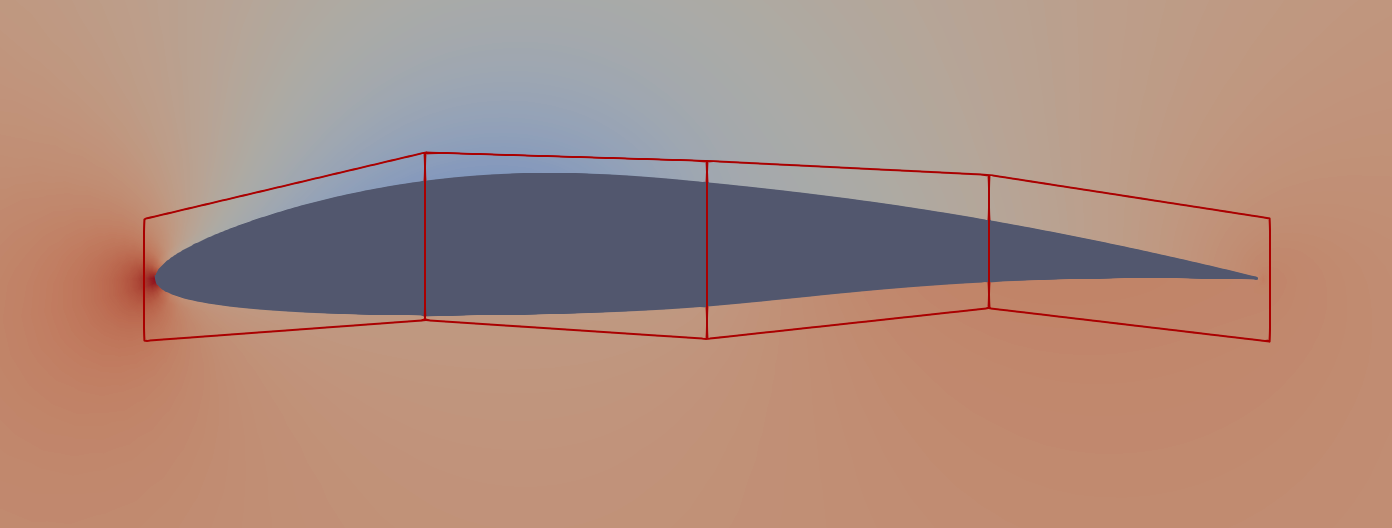
\includegraphics[width=0.9\linewidth]{images/deformed_FFD.png} 
    \caption{Deformed FFD points and airfoil shape at the last optimization iteration.}
  \end{figure}
  \end{frame}
%---------------------------------------------------------------%

%---------------------------------------------------------------%
\begin{frame}{}
  \center \Large Details of configuration files
\end{frame}
%---------------------------------------------------------------%

%---------------------------------------------------------------%
\begin{frame}[fragile]{Folders and files before the optimization }
  \footnotesize
  \begin{lstlisting}
  naca0012/incompressible
  |-- 0.orig // initial fields and boundary conditions
  |-- constant  // flow and turbulence property definition
  |-- FFD  // folder that contains the FFD file
  |-- profiles // naca0012 profile coordinate for mesh generation
  |-- system // flow discretization, setup, time step, etc
  |-- Allclean.sh // script to clean up the simulation results
  |-- genAirFoilMesh.py // python script called by preProcessing.sh
  |-- paraview.foam // dummy file for paraview post-processing
  |-- preProcessing.sh  // bash script to generate the mesh
  |-- runScript.py // main run script for optimization
  \end{lstlisting}
  \normalsize
  \vspace{-0.15in}
  NOTE: The \texttt{0}, \texttt{constant}, and \texttt{system} folders are OpenFOAM essential, and the rests are for DAFoam optimization
  \end{frame}
%---------------------------------------------------------------%

%---------------------------------------------------------------%
\begin{frame}[fragile]{Folders and files after the optimization }
\footnotesize
\begin{lstlisting}
naca0012/incompressible
|-- 0 // initial fields and boundary conditions
|-- 0.00000001  // flow solution for the baseline design
|-- 0.00000002  // flow solution for the 1st opt iteration
|-- 0.00000018  // flow solution for the final opt iteration
|-- constant  // flow and turbulence property definition
|-- FFD  // folder that contains the FFD file
|-- profiles // naca0012 profile coordinate for mesh generation
|-- system // flow discretization, setup, time step, etc
|-- Allclean.sh // script to clean up the simulation results
|-- deformedFFD_018.dat // deformed FFD points for the final opt iter 
|-- dRdWColoring_1.bin // computed coloring files
|-- DVConstraints.dat // visualization of constraints (Tecplot format)
|-- designVariableHist.txt // history of design variables during opt
|-- genAirFoilMesh.py // python script called by preProcessing.sh
|-- logMeshGeneration.txt // log file for mesh generation
|-- logOpt.txt // full log file for optimization
|-- objFuncHist.txt // objective history for ONE flow solution
|-- opt_IPOPT.txt // log file output by optimizer IPOPT
|-- paraview.foam // dummy file for paraview post-processing
|-- preProcessing.sh  // bash script to generate the mesh
|-- runScript.py // main run script for optimization
|-- totalDerivHist.txt // history of total derivative during opt
|-- surfaceMesh.xyz  // surface mesh generated by pyHyp
|-- volumeMesh.xyz   // volume mesh generated by pyHyp
\end{lstlisting}
\end{frame}
%---------------------------------------------------------------%

%---------------------------------------------------------------%
\begin{frame}[fragile]{The \texttt{0} folder (1/2)}
  The \texttt{0} folder contains files for all the state variables, and their initial and boundary values are defined in these files
  \small
  \begin{lstlisting}
  0
  |-- nut        // turbulence viscosity 
  |-- nuTilda    // working variable in the SA turbulence model
  |-- p          // pressure
  |-- U          // velocity
  |-- k          // k for SST turbulence model
  |-- omega      // omega for SST turbulence model
  |-- epsilon      // epsilon for kEpsilon turbulence model
  \end{lstlisting}
\end{frame}
%---------------------------------------------------------------%

%---------------------------------------------------------------%
\begin{frame}[fragile]{The \texttt{0} folder (2/2)}
  Open 0/U and check the initial and boundary conditions for velocity. Similarly, we need to define the conditions for all other variables

  \scriptsize
  \lstset{ language=C++ }
  \begin{lstlisting}
  // U magnitude 10 m/s. The internal and boundary field values defined in 0/U will be overwritten by DAFoam when running optimization. This is because we have define the boundary values in "primalBC"-"daOptions" of runScript.py
  internalField uniform (10 0 0);
  boundaryField
  {
      "(wing.*)"          // boundary patch name for wing*
      {
          type            fixedValue;      // boundary type
          value           uniform (0 0 0); // boundary value
      }
      symmetry1           // symmetry plane
      {
          type            symmetry;
      }
      symmetry2
      {
          type            symmetry;
      }
      inout               // far field, usually no need to change
      {
          type            inletOutlet; 
          inletValue      $internalField;
          value           $internalField;
      }
  }
  \end{lstlisting}
  
\end{frame}
%---------------------------------------------------------------%

%---------------------------------------------------------------%
\begin{frame}[fragile]{The \texttt{0.00000018} folder}
  Open 0.000000018/U.gz and check the final converged velocity field for the optimized design. NOTE: the \texttt{internalField} is no longer \texttt{uniform} as in the 0/U file.
  \scriptsize
  \begin{lstlisting}
    internalField   nonuniform List<vector>  // nonuniform internal field
    4032
    (
    (3.9243226 -1.290095 -0.0028988106)
    (3.7305871 -0.99840567 -0.0027730653)
    (3.554621 -1.3012481 -0.0028666955)
    (3.8325503 -0.95915536 -0.003049858)
    (3.947682 -0.94315159 -0.0028641267)
    (4.2338067 -1.0326866 -0.0031121561)
    (2.738578 -0.99318945 -0.0026861221)
    (3.2447924 -0.87974595 -0.0029403715)
    (4.3552657 -0.78274271 -0.0032382407)
    (3.9498574 -0.91532577 -0.0028354695)
    (4.5629592 -1.0266758 -0.0031897207)
    (4.8687782 -0.9436423 -0.0033734098)
    (3.6192063 -0.29059501 -0.0019943858)
    .....
  \end{lstlisting}
  \normalsize
  NOTE: The \texttt{0.00000018} folder also contains the optimized (deformed) mesh points in 0.00000018/constant/polyMesh/points.gz, which is different from the baseline mesh points in constant/polyMesh/points.gz (see next slide)
  
\end{frame}
%---------------------------------------------------------------%



%---------------------------------------------------------------%
\begin{frame}[fragile]{The \texttt{constant} folder (1/3)}
  The \texttt{constant} folder contains mesh, flow and turbulence property definitions.
  \small
  \begin{lstlisting}
  constant
  |-- polyMesh   // mesh points, faces, and boundary info
      |-- boundary      // mesh boundary patch names and types
      |-- faces.gz      // mesh faces 
      |-- neighbour.gz  // face neighbour info
      |-- owner.gz      // face owner info
      |-- points.gz     // baseline mesh point coordinates
  |-- transportProperties  // flow properties
  |-- turbulenceProperties // turbulence model
  \end{lstlisting}

\end{frame}
%---------------------------------------------------------------%

%---------------------------------------------------------------%
\begin{frame}[fragile]{The \texttt{constant} folder (2/3)}
  The \texttt{bounary} file defines the name and type of the boundary patches
  \scriptsize
  \begin{lstlisting}
  5 // number of boundary patches
  (
      symmetry1    // name of the mesh boundary patch, symmetry plane
      {
          type            symmetry;  // type of the boundary patch
          nFaces          4032;      // number of faces in the patch
          startFace       7938;     // start face
      }
      wing    // wing surface
      {
          type            wall;
          nFaces          126;
          startFace       16002;
      }
      inout  // far field
      {
          type            patch;
          nFaces          126;
          startFace       16128;
      }
      ...
  )
  \end{lstlisting}

\end{frame}
%---------------------------------------------------------------%


%---------------------------------------------------------------%
\begin{frame}[fragile]{The \texttt{constant} folder (3/3)}
  The \texttt{transportProperties} file defines flow properties
  \small
  \begin{lstlisting}
  transportModel Newtonian;
  nu 1.5e-5;  // define the molecular viscosity
  \end{lstlisting}

  \normalsize
  The \texttt{turbulenceProperties} file defines turbulence model 
  \small
  \begin{lstlisting}
  simulationType RAS;  // RAS=RANS in OpenFOAM 
  RAS 
  { 
      RASModel       SpalartAllmaras;  // the SA turbulence model
      turbulence     on;
      printCoeffs    off;
  } 
  \end{lstlisting}

\end{frame}
%---------------------------------------------------------------%

%---------------------------------------------------------------%
\begin{frame}[fragile]{The \texttt{system} folder (1/5)}
  The \texttt{system} folder contains
  \footnotesize
  \begin{lstlisting}
  system
  |-- controlDict    // defines system parameters such as time step
  |-- createPatchDict // parameters used by the createPatch utility 
  |-- decomposeParDict // mesh decomposition parameters for parallel run
  |-- fvSchemes  // discretization schemes
  |-- fvSolution // linear equation solution strategy
  \end{lstlisting}
  
\end{frame}
%---------------------------------------------------------------%

%---------------------------------------------------------------%
\begin{frame}[fragile]{The \texttt{system} folder (2/5)}
  The \texttt{control} file contains flow setup such as step size
  \footnotesize
  \begin{lstlisting}
  startFrom       startTime;   // simulation starts from startTime
  startTime       0;           // if startFrom=startTime, define it here
  stopAt          endTime;     // simulation ends at endTime
  endTime         1000;        // define endTime here
  deltaT          1;           // time step
  writeControl    timeStep;    // how to write the results
  writeInterval   1000;        // write flow field every 1000 steps
  purgeWrite      0;           // whether to purge intermediate output
  writeFormat     ascii;       // binary or ascii output format
  writePrecision  8;           // Write precision for data output
  writeCompression on;         // Compress the output files with .gz format
  timeFormat      general;     // time format
  timePrecision   8;           // time IO accuracy
  runTimeModifiable true;      // Allow modification during runtime
  // Do not print solver performance from OpenFOAM, the information 
  // printed to the screen will be completely controlled by DAFoam
  DebugSwitches
  {
    SolverPerformance 0;       
  }
  \end{lstlisting}
  
\end{frame}
%---------------------------------------------------------------%

%---------------------------------------------------------------%
\begin{frame}[fragile]{The \texttt{system} folder (3/5)}
  The \texttt{decomposeParDict} contains parallel run setup. NOTE: there is no need to manually change this file, because it will be automatically generated by DAFoam when the optimization runs.
  \small
  \begin{lstlisting}
  numberOfSubdomains     4;  // number of decomposed domain
  method             scotch;
  \end{lstlisting}
  
\end{frame}
%---------------------------------------------------------------%


%---------------------------------------------------------------%
\begin{frame}[fragile]{The \texttt{system} folder (4/5)}
  The \texttt{fvSchemes} file contains discretization definition for each variable
  \scriptsize
  \begin{lstlisting}
  ddtSchemes 
  {
      default                                   steadyState;
  }
  gradSchemes
  {
      default                                   Gauss linear;
  }
  divSchemes // NOTE: need to specify divergence discretization for each variable
  {
      default                                   none;
      div(phi,U)                                bounded Gauss linearUpwindV grad(U);
      div(phi,nuTilda)                          bounded Gauss upwind;
      div((nuEff*dev2(T(grad(U)))))             Gauss linear;
      div((-devRhoReff.T()&U))                  Gauss linear;
  }
  interpolationSchemes
  {
      default                                   linear;
  }
  laplacianSchemes
  {
      default                                   Gauss linear corrected;
  }
  \end{lstlisting}
  
\end{frame}
%---------------------------------------------------------------%

%---------------------------------------------------------------%
\begin{frame}[fragile]{The \texttt{system} folder (5/5)}
  The \texttt{fvSolution} file contains strategy for linear equation solution
  \scriptsize
  \begin{lstlisting}
  SIMPLE
  {
      consistent                         false; // don't use SIMPLEC
      nNonOrthogonalCorrectors           0;
  }
  solvers
  {
      "(p|p_rgh|G)" // linear GaussSeideil solver for p equations
      {
          solver                         GAMG;
          smoother                       GaussSeidel;
          relTol                         0.1;
          tolerance                      0;
      }
  }
  relaxationFactors // NOTE: need to specify relaxation for each variable
  {
      fields
      {
          "(p|p_rgh)"                    0.30;
      }
      equations
      {
          "(U|T|e|h|nuTilda|k|epsilon|omega)" 0.70;
      }
  }

  \end{lstlisting}
  
\end{frame}
%---------------------------------------------------------------%


%---------------------------------------------------------------%
\begin{frame}[fragile]{The \texttt{preProcessing.sh} script (1/4)}
  The \texttt{preProcessing.sh} script is used to generate mesh. We first run genAirFoilMesh.py to read the airfoil coordinates from the profiles folder and generate structured mesh using pyHyp and output the mesh as volumeMesh.xyz. 
  \scriptsize
  \lstset{ language=bash }
  \begin{lstlisting}
  python genAirFoilMesh.py > log.meshGeneration
  \end{lstlisting}

  \vspace{-0.1in}
  \normalsize
  The \texttt{genAirFoilMesh.py} script reads:
  \scriptsize
  \lstset{ language=bash }
  \begin{lstlisting}
  ########## user input ################
  prefix = "./profiles/"
  airfoilProfilePS = prefix + "NACA0012PS.profile"
  airfoilProfileSS = prefix + "NACA0012SS.profile"
  ZSpan = 0.1  # width in the z direction
  nSpan = 2  # how many points in z
  # PS parameters
  dX1PS = 0.005  # first dx from the LE
  Alpha1PS = 1.2  # clustering from the LE
  dX2PS = 2e-3  # first dx from the TE
  Alpha2PS = 1.2  # clustering from the TE
  dXMaxPS = 0.02  # max dx for PS
  ...
  # TE parameters
  NpTE = 5  # number of points for blunt TE
  # 3D
  NpExtrude = 33  # how many points to extrude for the 3D volume mesh
  yWall = 4e-3  # first layer mesh length
  marchDist = 20.0  # march distance for extruding
  \end{lstlisting}

\end{frame}
%---------------------------------------------------------------%

%---------------------------------------------------------------%
\begin{frame}[fragile]{The \texttt{preProcessing.sh} script (2/4)}
  Then, we use the plot3dToFoam utility to convert the plot3D mesh volumeMesh.xyz to OpenFOAM format and store the mesh in \texttt{constant/polyMesh}
  \footnotesize
  \lstset{ language=bash }
  \begin{lstlisting}
  plot3dToFoam -noBlank volumeMesh.xyz >> log.meshGeneration
  \end{lstlisting}
  \normalsize
  After running the above command, the volumeMesh.xyz will be converted to the OpenFOAM mesh. However, in the boundary patch file \texttt{constant/polyMesh/boundary}, there is only one boundary patch, and reads:

  \footnotesize
  \lstset{ language=bash }
  \begin{lstlisting}
  1
  (
      defaultFaces
      {
          type            wall;
          inGroups        1(wall);
          nFaces          9324;
          startFace       8946;
      }
  )
  \end{lstlisting}


\end{frame}
%---------------------------------------------------------------%


%---------------------------------------------------------------%
\begin{frame}[fragile]{The \texttt{preProcessing.sh} script (3/4)}
  Then, we run autoPatch to automatically split the boundary patches. Here the argument 60 means split the mesh based on 60 degree feature angle (lower this value will generate more patches). Essentially, this call will modify the \texttt{constant/polyMesh/boundary} file and generate new patches called auto0, auto1, auto2, etc.
  \scriptsize
  \lstset{ language=bash }
  \begin{lstlisting}
  autoPatch 60 -overwrite >> log.meshGeneration
  \end{lstlisting}

  \vspace{-0.1in}
  \normalsize
  Once done, \texttt{constant/polyMesh/boundary} reads:

  \scriptsize
  \lstset{ language=bash }
  \begin{lstlisting}
6
(
    ...
    auto0
    {
        type            patch;
        nFaces          4536;
        startFace       8946;
    }
    ...
    auto4
    {
        type            patch;
        nFaces          4536;
        startFace       13482;
    }
)
  \end{lstlisting}


\end{frame}
%---------------------------------------------------------------%


%---------------------------------------------------------------%
\begin{frame}[fragile]{The \texttt{preProcessing.sh} script (4/4)}
  The above generated boundary file has boundary names such as auto0, auto1, auto2, etc. Now group and rename the above generated patches to meaningful names, e.g. wing, symmetry, etc, see system/createPathDict
  \footnotesize
  \lstset{ language=bash }
  \begin{lstlisting}
  createPatch -overwrite >> log.meshGeneration
  \end{lstlisting}
  \vspace{-0.1in}
  \normalsize
  \texttt{system/createPathDict} reads:

  \footnotesize
  \lstset{ language=c++ }
  \begin{lstlisting}
patches
(
    ...
    {   
        name wing; // Name of new patch
        patchInfo // Dictionary to construct new patch from
        {
            type wall;
        }
        // How to construct: either from 'patches' or 'set'
        constructFrom patches;
        // which patches to group and renamed as "wing"
        patches (auto2 auto3);
    }
    ...
);
  \end{lstlisting}


\end{frame}
%---------------------------------------------------------------%


%---------------------------------------------------------------%
\begin{frame}[fragile]{The airfoil coordinates}
\small
  When running the above \texttt{genAirFoilMesh.py} script, it will look for the airfoil coordinates in the \texttt{profiles} folder. NOTE: We need to define the upper profile (SS; suction side) and lower profile (PS; pressure side) separately. The range of x needs to be from 0 to 1. And we need to manually delete the last few points to make a blunt trailing edge. In other words, the last point should have x$\approx$0.999, instead of 1.0

  \scriptsize
  \lstset{ language=bash }
  \begin{lstlisting}
 NACA0012SS.profile
 0.0000000 0.0000000 # coordinate should start from 1
 0.0005839 -.0042603
 0.0023342 -.0084289
 ...
 0.9947532 -.0019938
 0.9976658 -.0015870
 0.9994161 -.0013419 # end at about 0.999; we have deleted the last few points
  \end{lstlisting}
  \normalsize

  \scriptsize
  \lstset{ language=bash }
  \begin{lstlisting}
 NACA0012PS.profile
 0.0000000 0.0000000 # coordinate should start from 1
 0.0005839 0.0042603
 0.0023342 0.0084289
 ...
 0.9947532 0.0019938
 0.9976658 0.0015870
 0.9994161 0.0013419 # end at about 0.999; we have deleted the last few points
  \end{lstlisting}

\end{frame}
%---------------------------------------------------------------%

%---------------------------------------------------------------%
\begin{frame}[fragile]{The \texttt{FFD} folder}

  We use the \texttt{FFD/genFFD.py} script to generate the FFD points and save it in the plot3D format (FFD/wingFFD.xyz). 
  
  \footnotesize
  \lstset{ language=bash }
  \begin{lstlisting}
  nBlocks = 1  # we only have one FFD block
  nx = [5]  # number of FFD points in the x direction
  ny = [2]
  nz = [2]
  # we need to define the coordinates for the 8 corner points and the 
  # rest of points will be automatically generated by this script.
  corners[0,0,:] = [-0.010,-.0700,0.0]
  corners[0,1,:] = [-0.010,-0.0700,0.1]
  corners[0,2,:] = [-0.010,0.0700,0.0]
  corners[0,3,:] = [-0.010,0.0700,0.1]
  corners[0,4,:] = [ 1.01,-.07,0.0]
  corners[0,5,:] = [ 1.01,-.07,0.10]
  corners[0,6,:] = [ 1.01,0.07,0.0]
  corners[0,7,:] = [ 1.01,0.07,0.1]
  \end{lstlisting}
  
  \normalsize
  Paraview has problems loading small plot3D files, so we can convert it to Tecplot format by running this command. Then we can load wingFFD.dat in Paraview.

  \footnotesize
  \lstset{ language=bash }
  \begin{lstlisting}
  dafoam_plot3d2tecplot.py wingFFD.xyz wingFFD.dat
  \end{lstlisting}


\end{frame}
%---------------------------------------------------------------%


%---------------------------------------------------------------%
\begin{frame}[fragile]{Visualize the FFD points (wingFFD.dat) in Paraview}
  The FFD points have to completely contain the design surface!!
  \begin{figure}
  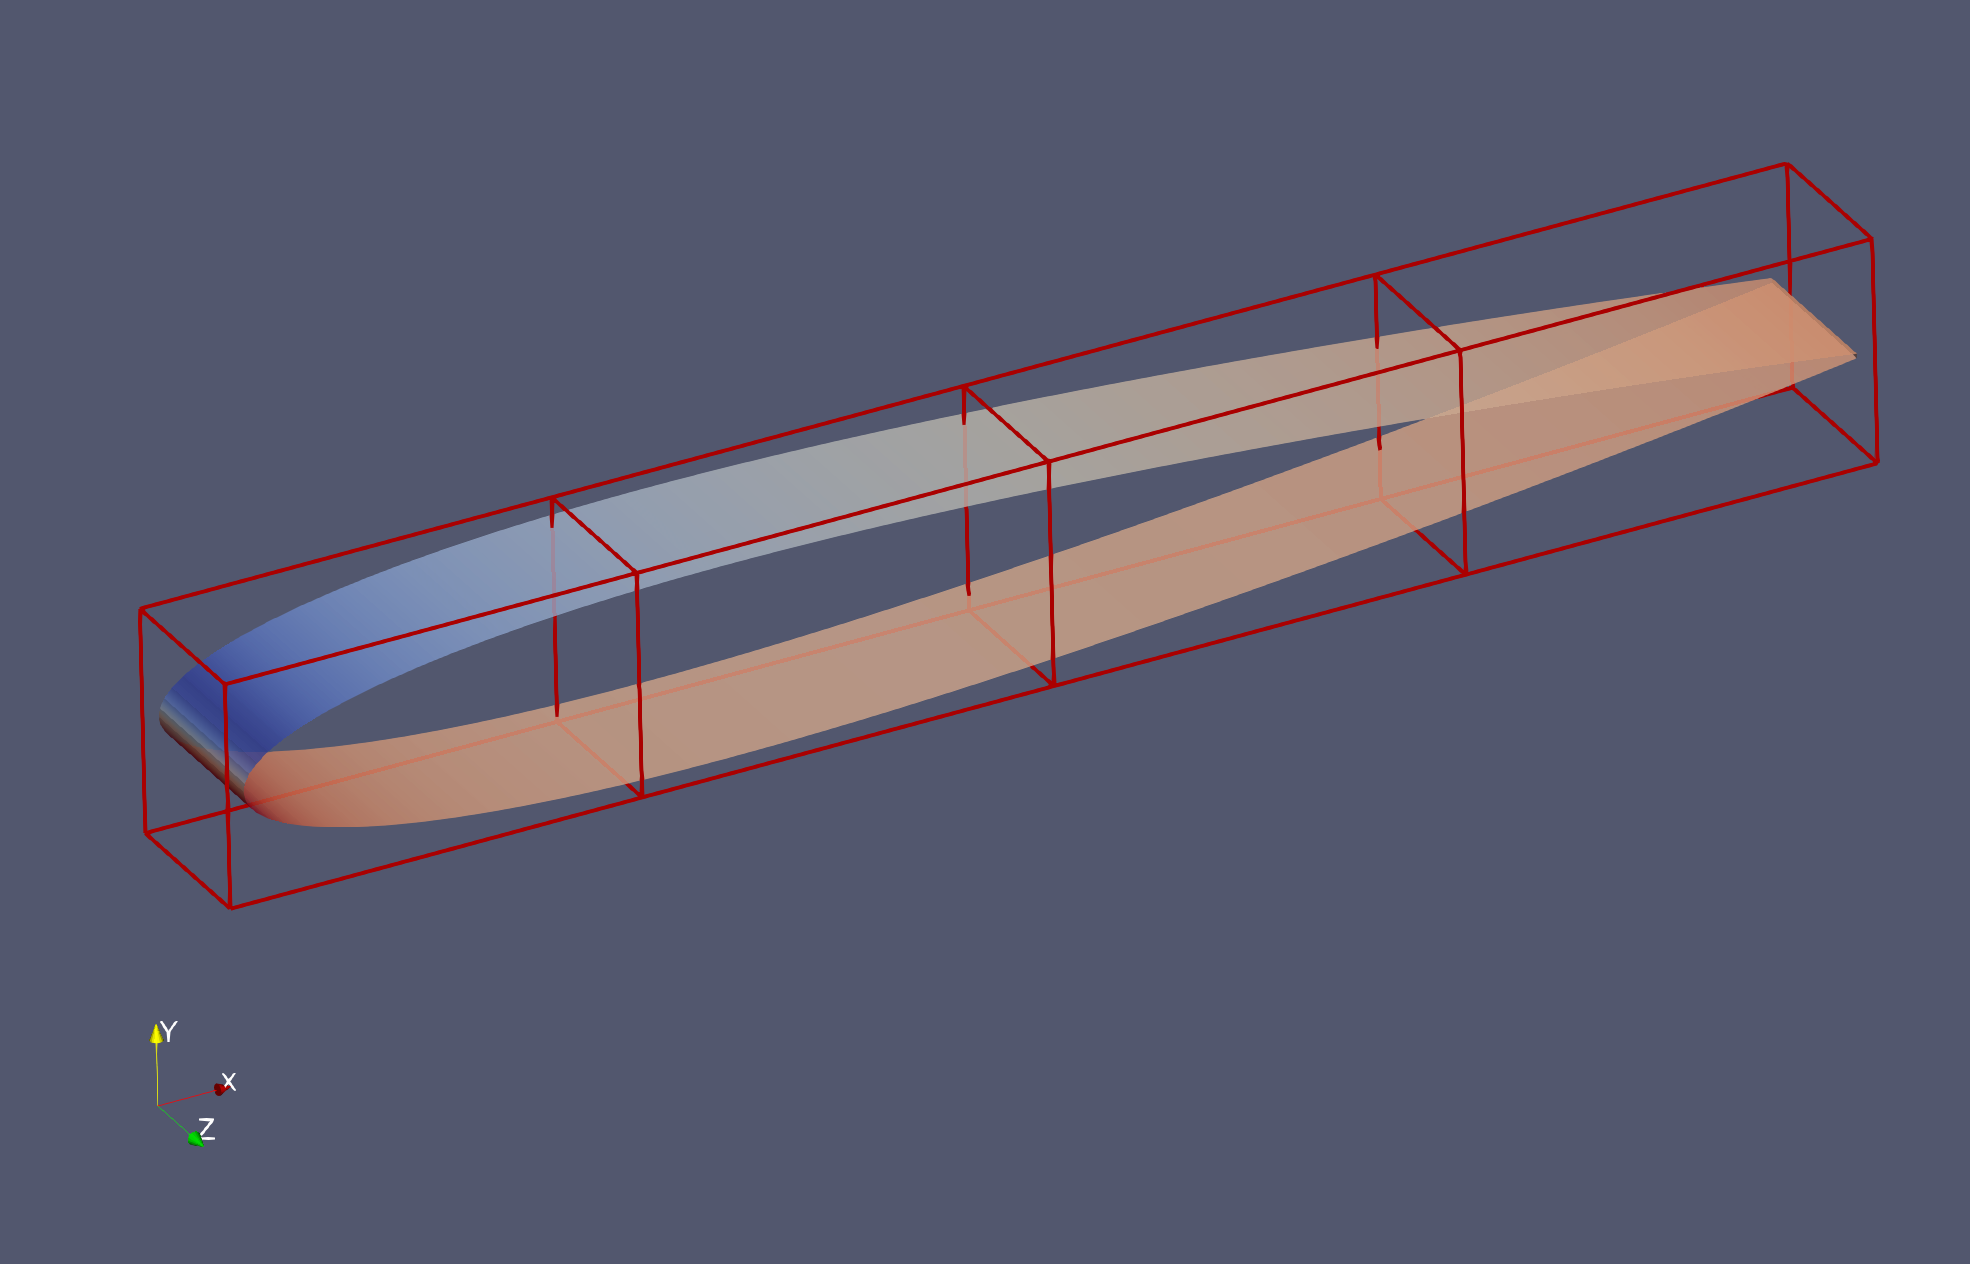
\includegraphics[width=0.95\linewidth]{images/genFFD.png} 
  \end{figure}
\end{frame}
%---------------------------------------------------------------%


%---------------------------------------------------------------%
\begin{frame}[fragile]{The \texttt{runScript.py} script (1/11)}

  \scriptsize
  \lstset{ language=python }
  \begin{lstlisting}
# ================
# Input Parameters
# ================
parser = argparse.ArgumentParser()
# we support slsqp, ipopt, and snopt
parser.add_argument("--opt", help="optimizer to use", type=str, default="ipopt")
# the default task is optimization (opt), we can also do runPrimal, runAjoint, verifySens, etc.
parser.add_argument("--task", help="type of run to do", type=str, default="opt")
args = parser.parse_args()
gcomm = MPI.COMM_WORLD

# Define the global parameters here
U0 = 10.0  # far field velocity
p0 = 0.0  # far field pressure (relative to the ref value)
nuTilda0 = 4.5e-5  # far field turbulence variables
k0 = 0.015  
epsilon0 = 0.14
omega0 = 100.0
CL_target = 0.5  # target lift coefficient for optimization
alpha0 = 5.0   # guess of angle of attack for CL_target
A0 = 0.1  # reference area for normalizing lift and drag
  \end{lstlisting}
\end{frame}
%---------------------------------------------------------------%

%---------------------------------------------------------------%
\begin{frame}[fragile]{The \texttt{runScript.py} script (2/11)}

  \scriptsize
  \lstset{ language=python }
  \begin{lstlisting}
daOptions = {
    "designSurfaces": ["wing"],  # design surface names
    "solverName": "DASimpleFoam",  # solver name
    "adjJacobianOption": "JacobianFree",  # Use Jacobian-free adjoint with AD
    "primalMinResTol": 1.0e-8,  # flow solution residual tolerance
    "primalBC": {  # set boundary condition here and overwrite 0/U, 0/p, etc.
        "U0": {"variable": "U", "patches": ["inout"], "value": [U0, 0.0, 0.0]},
        "p0": {"variable": "p", "patches": ["inout"], "value": [p0]},
        ...
        "useWallFunction": True,  # use wall functions for turbulence variables
    },
    "objFunc": {  # define objective function here
        "CD": {  # first objective name is CD
            "part1": {
                "type": "force",  # it is of "force" type
                "source": "patchToFace",  # force is computed from selected patches
                "patches": ["wing"],  # patch names for force computation
                "directionMode": "parallelToFlow",  # force dir is parallel to flow
                "alphaName": "alpha",  # provide angle of attack name for force dir
                "scale": 1.0 / (0.5 * U0 * U0 * A0),  # scale to normalize force
                "addToAdjoint": True,  # whether to compute adjoint for this objFunc
            }
        },
        "CL": {  # second objective name is CL
                ...
                "directionMode": "normalToFlow",  # force dir is normal to flow
                ...
        },
    },
  \end{lstlisting}
\end{frame}
%---------------------------------------------------------------%

%---------------------------------------------------------------%
\begin{frame}[fragile]{The \texttt{runScript.py} script (3/11)}

  \scriptsize
  \lstset{ language=python }
  \begin{lstlisting}
daOptions = {
    ...
    "adjEqnOption": {  # adjoint solution options
        "gmresRelTol": 1.0e-8,  # adjoint solutioin residual tolerance
        "pcFillLevel": 1,   # preconditioner fill-in level
        "jacMatReOrdering": "rcm"  # preconditioner re-ordering
    },
    "normalizeStates": {  # state variable normalization values for adjoint
        "U": U0,  # far field velocity to normalize U
        "p": U0 * U0 / 2.0,  # dynamic pressure to normalize p (incompressible)
        "nuTilda": nuTilda0 * 10.0,
        "k": k0 * 10.0,
        "epsilon": epsilon0,
        "omega": omega0,
        "phi": 1.0,  # always use 1.0 to normalize ph
    },
    # finite-difference step size for computing preconditioner
    "adjPartDerivFDStep": {"State": 1e-7, "FFD": 1e-3},
    # how frequent to recompute the preconditioner dRdWTPC
    "adjPCLag": 100,
    # provide an empty key for place holder (values to be assigned later)
    "designVar": {},
    # write the deformed FFD files during optimization
    "writeDeformedFFDs": True
}
  \end{lstlisting}

  NOTE: A complete list of daOptions are at: \\ \url{https://dafoam.github.io/doxygen/html/classdafoam_1_1pyDAFoam_1_1DAOPTION.html}
\end{frame}
%---------------------------------------------------------------%

%---------------------------------------------------------------%
\begin{frame}[fragile]{The \texttt{runScript.py} script (4/11)}

  \scriptsize
  \lstset{ language=python }
  \begin{lstlisting}
# mesh warping parameters, users need to manually specify the symmetry plane and their normals
meshOptions = {
    "gridFile": os.getcwd(),
    "fileType": "openfoam",
    # point and normal for the symmetry plane
    "symmetryPlanes": [[[0.0, 0.0, 0.0], [0.0, 0.0, 1.0]], [[0.0, 0.0, 0.1], [0.0, 0.0, 1.0]]],
}

# options for optimizers
if args.opt == "snopt":
    optOptions = {
        ...
    }
elif args.opt == "ipopt":
    optOptions = {
        "tol": 1.0e-6,  # optimality
        "constr_viol_tol": 1.0e-6,  # feasibility tolerance
        "max_iter": 50,  # max number of optimization iterations
        "print_level": 5,
        "output_file": "opt_IPOPT.txt",
        "mu_strategy": "adaptive",
        "limited_memory_max_history": 10,
        "nlp_scaling_method": "none",
        "alpha_for_y": "full",
        "recalc_y": "yes",
    }
...
}
  \end{lstlisting}

\end{frame}
%---------------------------------------------------------------%

%---------------------------------------------------------------%
\begin{frame}[fragile]{The \texttt{runScript.py} script (5/11)}

  \scriptsize
  \lstset{ language=python }
  \begin{lstlisting}
# ========================
# Design variable setup
# ========================
def alpha(val, geo):  # define the angle of attack function to update primalBC
    aoa = val[0] * np.pi / 180.0  # val[0] is the aoa in degree
    inletU = [float(U0 * np.cos(aoa)), float(U0 * np.sin(aoa)), 0] # U components
    DASolver.setOption("primalBC", {"U0": {"variable": "U", "patches": ["inout"], 
        "value": inletU}})  # update U in primalBC based on aoa 
    DASolver.updateDAOption() # update the value in the C++ layer
DVGeo = DVGeometry("./FFD/wingFFD.xyz")  # read the FFD point
DVGeo.addRefAxis("bodyAxis", xFraction=0.25, alignIndex="k")  # add ref axis
# select points
iVol = 0  # we only have one FFD block, so it is the 0th index
pts = DVGeo.getLocalIndex(iVol)  # get all the FFD points
indexList = pts[:, :, :].flatten()  # select all the FFD points [:,:,:]
PS = geo_utils.PointSelect("list", indexList)
# shape variables that move in the y direction within [-1.0:1.0]
DVGeo.addGeoDVLocal("shapey", lower=-1.0, upper=1.0, axis="y", scale=1.0, pointSelect=PS)  # assign the PS to pointSelect
# update daOptions, the type of shape design variable is "FFD"
daOptions["designVar"]["shapey"] = {"designVarType": "FFD"} 
# angle of attack variable defined by the alpha(val, geo) function above
DVGeo.addGeoDVGlobal("alpha", value=[alpha0], func=alpha, lower=0.0, upper=10.0, scale=1.0) # initial aoa is [alpha0] and the bounds are [0:10]
# update daOptions, the type of aoa design variable is "AOA", we also need to 
# give patch names, flowAxis, and normalAxis to determine the force direction
daOptions["designVar"]["alpha"] = {"designVarType": "AOA", "patches": ["inout"], 
    "flowAxis": "x", "normalAxis": "y"} 
  \end{lstlisting}

\end{frame}
%---------------------------------------------------------------%


%---------------------------------------------------------------%
\begin{frame}[fragile]{The \texttt{runScript.py} script (6/11)}
  No need to change this part
  \scriptsize
  \lstset{ language=python }
  \begin{lstlisting}
# ======================
# DAFoam initialization
# ======================
DASolver = PYDAFOAM(options=daOptions, comm=gcomm)
DASolver.setDVGeo(DVGeo)
mesh = USMesh(options=meshOptions, comm=gcomm)
DASolver.addFamilyGroup(DASolver.getOption("designSurfaceFamily"), DASolver.getOption("designSurfaces"))
DASolver.printFamilyList()
DASolver.setMesh(mesh)
evalFuncs = []
DASolver.setEvalFuncs(evalFuncs)
  \end{lstlisting}

\end{frame}
%---------------------------------------------------------------%


%---------------------------------------------------------------%
\begin{frame}[fragile]{The \texttt{runScript.py} script (7/11)}
  \scriptsize
  \lstset{ language=python }
  \begin{lstlisting}
# ==================
# Constraint setup
# ==================
DVCon = DVConstraints()
DVCon.setDVGeo(DVGeo)
DVCon.setSurface(DASolver.getTriangulatedMeshSurface(groupName=DASolver.getOption("designSurfaceFamily")))
# leading and trailing edge lines for volume and thickness constraints
leList = [[1e-4, 0.0, 1e-4], [1e-4, 0.0, 0.1 - 1e-4]] # RED line
teList = [[0.998 - 1e-4, 0.0, 1e-4], [0.998 - 1e-4, 0.0, 0.1 - 1e-4]] # BLUE line
\end{lstlisting}
\vspace{-0.15in}
\begin{figure}
  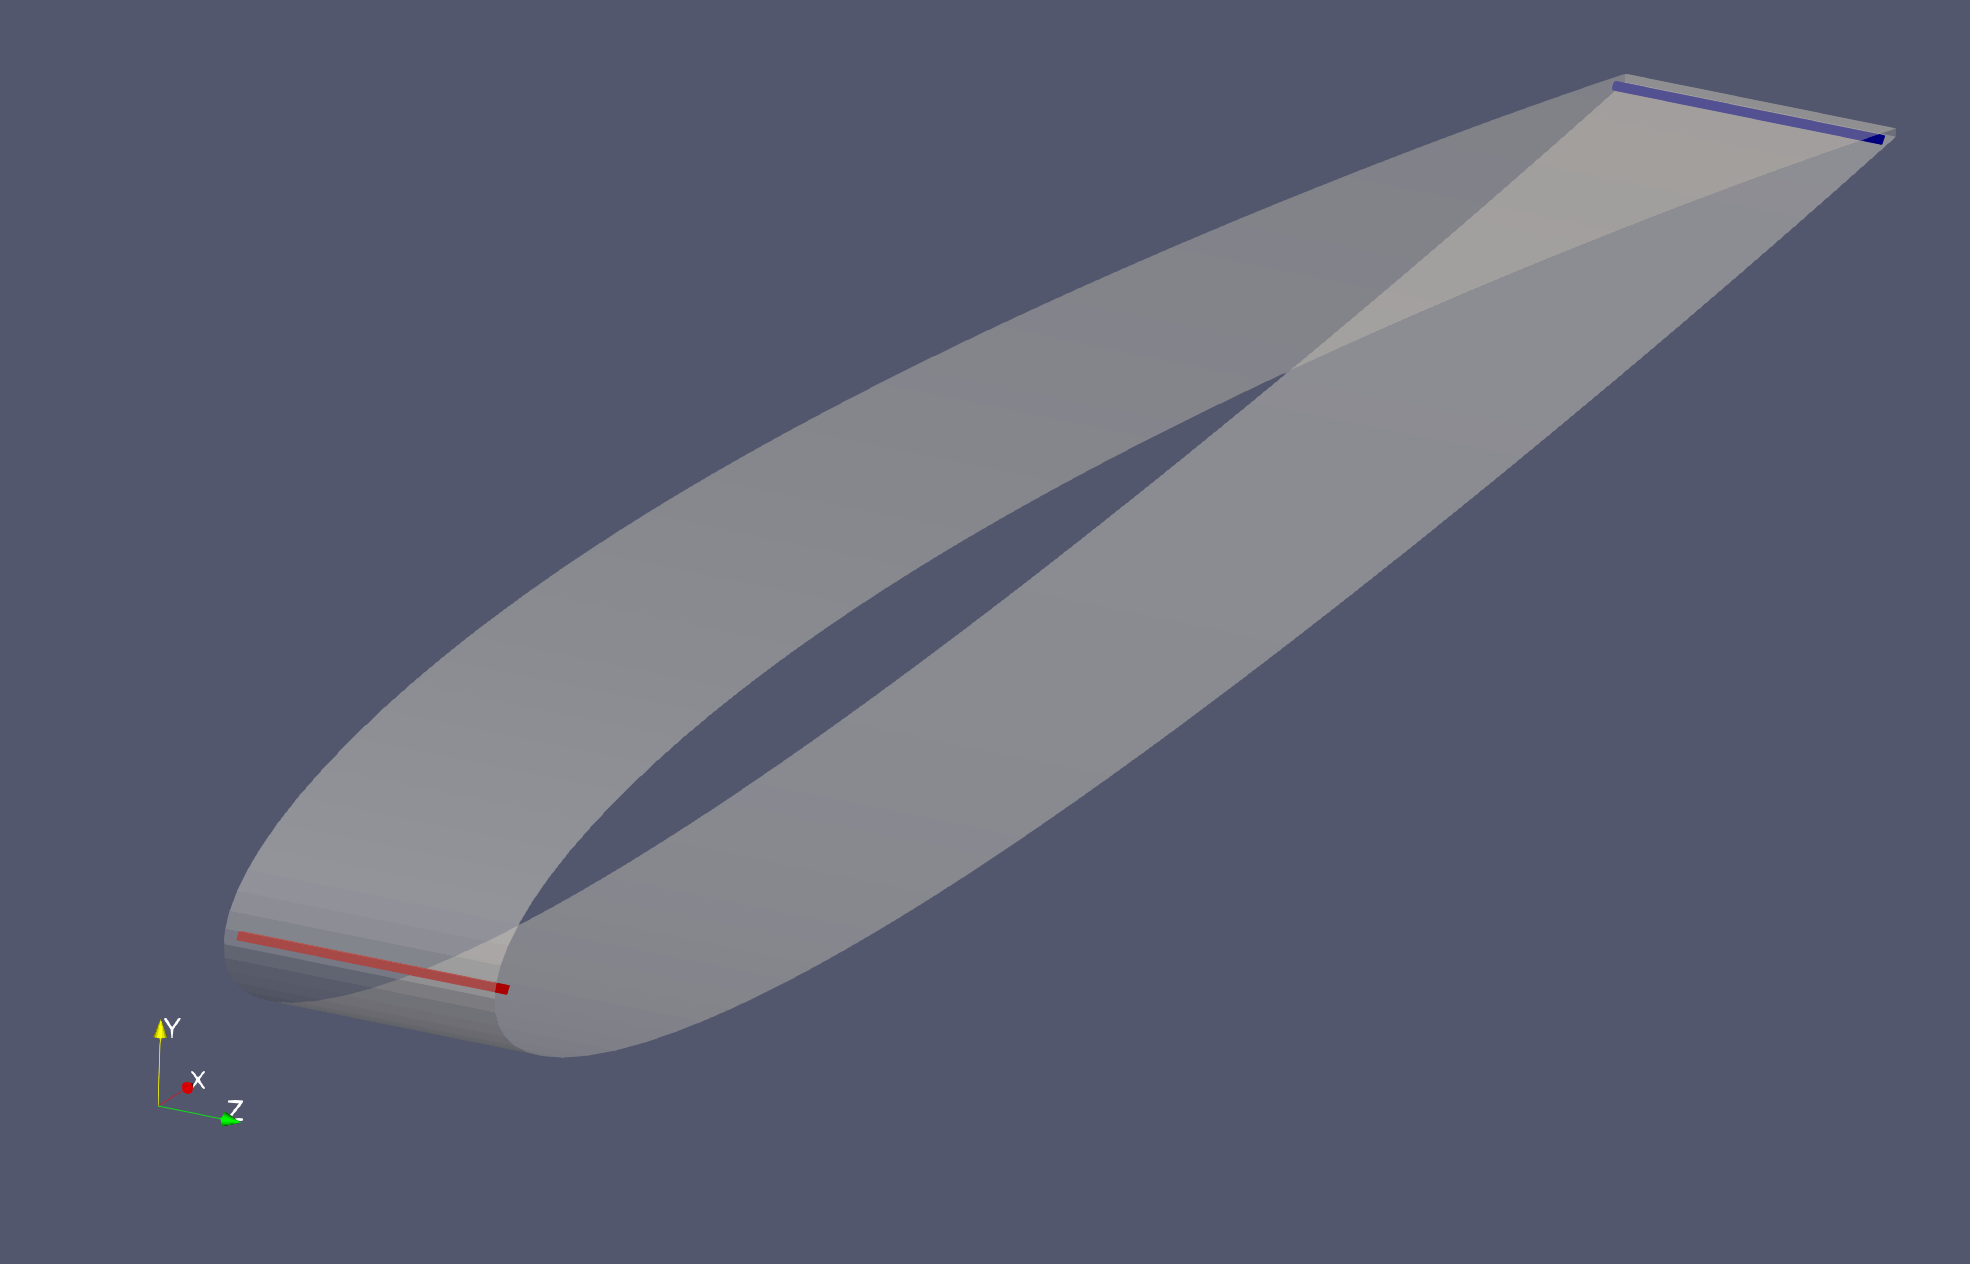
\includegraphics[width=0.7\linewidth]{images/LETE.png} 
\end{figure}

\end{frame}
%---------------------------------------------------------------%

%---------------------------------------------------------------%
\begin{frame}[fragile]{The \texttt{runScript.py} script (8/11)}

  \scriptsize
  \lstset{ language=python }
  \begin{lstlisting}
# volume constraint, we use the leList and teList as outer boundary and
# create 2x10 sample points defined by nSpan and nChord. Then, we project
# and these samle points to the airfoil surface to form trapezoid volumes
# the sum of these volumes is an approximated volume for the airfoil. 
# We constrain the relative upper and lower bounds [1.0:3.0] 
# based on the initial volume
DVCon.addVolumeConstraint(leList, teList, nSpan=2, nChord=10, lower=1.0, upper=3, scaled=True)

# thickness constraint, we use the leList and teList as outer boundary and
# create 2x10 sample points defined by nSpan and nChord. Then, we project
# and these samle points to the airfoil surface. The lengths of the projection
# lines are the local thickness of the airfoil. We constrain the relative
# upper and lower bounds [0.8:3.0] based on the initial local thickness
DVCon.addThicknessConstraints2D(leList, teList, nSpan=2, nChord=10, lower=0.8, upper=3.0, scaled=True)
\end{lstlisting}
\vspace{-0.2in}
\begin{figure}
  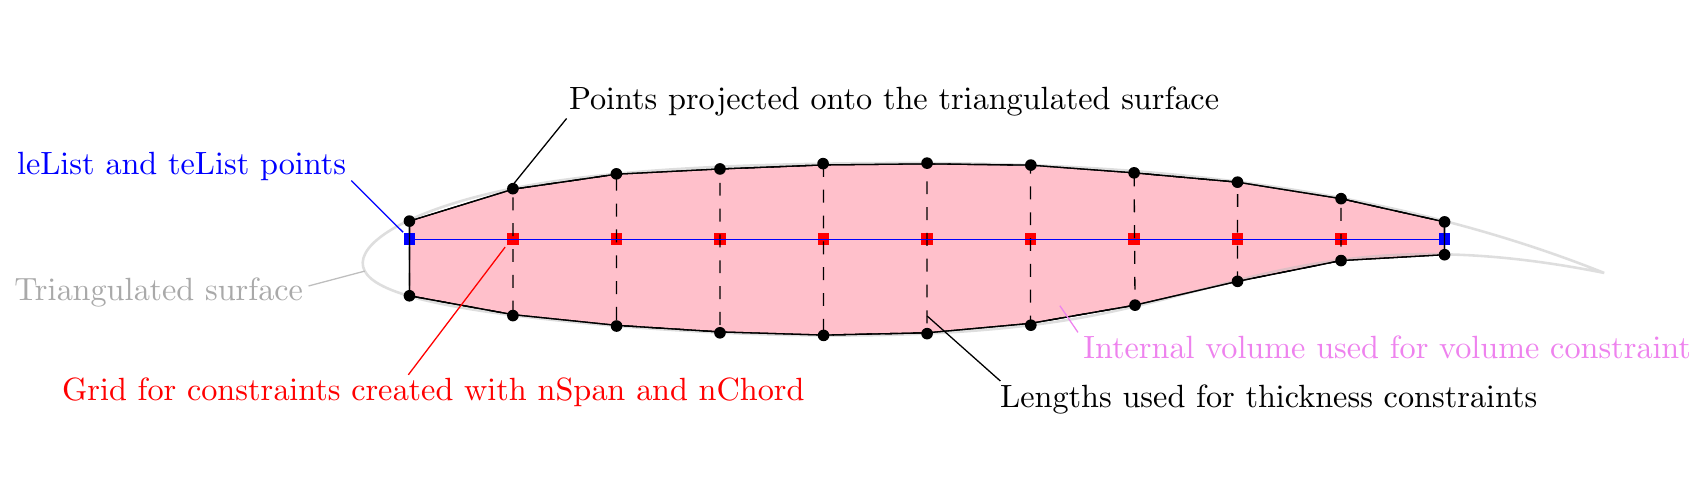
\includegraphics[width=\linewidth]{images/opt_thickness_and_vol_diagram.png} 
  \caption{Diagram for volume and thickness constraints.}
\end{figure}

\end{frame}
%---------------------------------------------------------------%

%---------------------------------------------------------------%
\begin{frame}[fragile]{The \texttt{runScript.py} script (9/11)}

  \scriptsize
  \lstset{ language=python }
  \begin{lstlisting}
# Create linear constraints to link the shape change between k=0 and k=1
nFFDs_x = pts.shape[0] # the x size of pts array
indSetA = []
indSetB = []
for i in range(nFFDs_x):
    for j in [0, 1]:
        indSetA.append(pts[i, j, 1]) # linking k=0 and k=1
        indSetB.append(pts[i, j, 0])
DVCon.addLinearConstraintsShape(indSetA, indSetB, factorA=1.0, factorB=-1.0, lower=0.0, upper=0.0)
\end{lstlisting}
\vspace{-0.2in}
\begin{figure}
  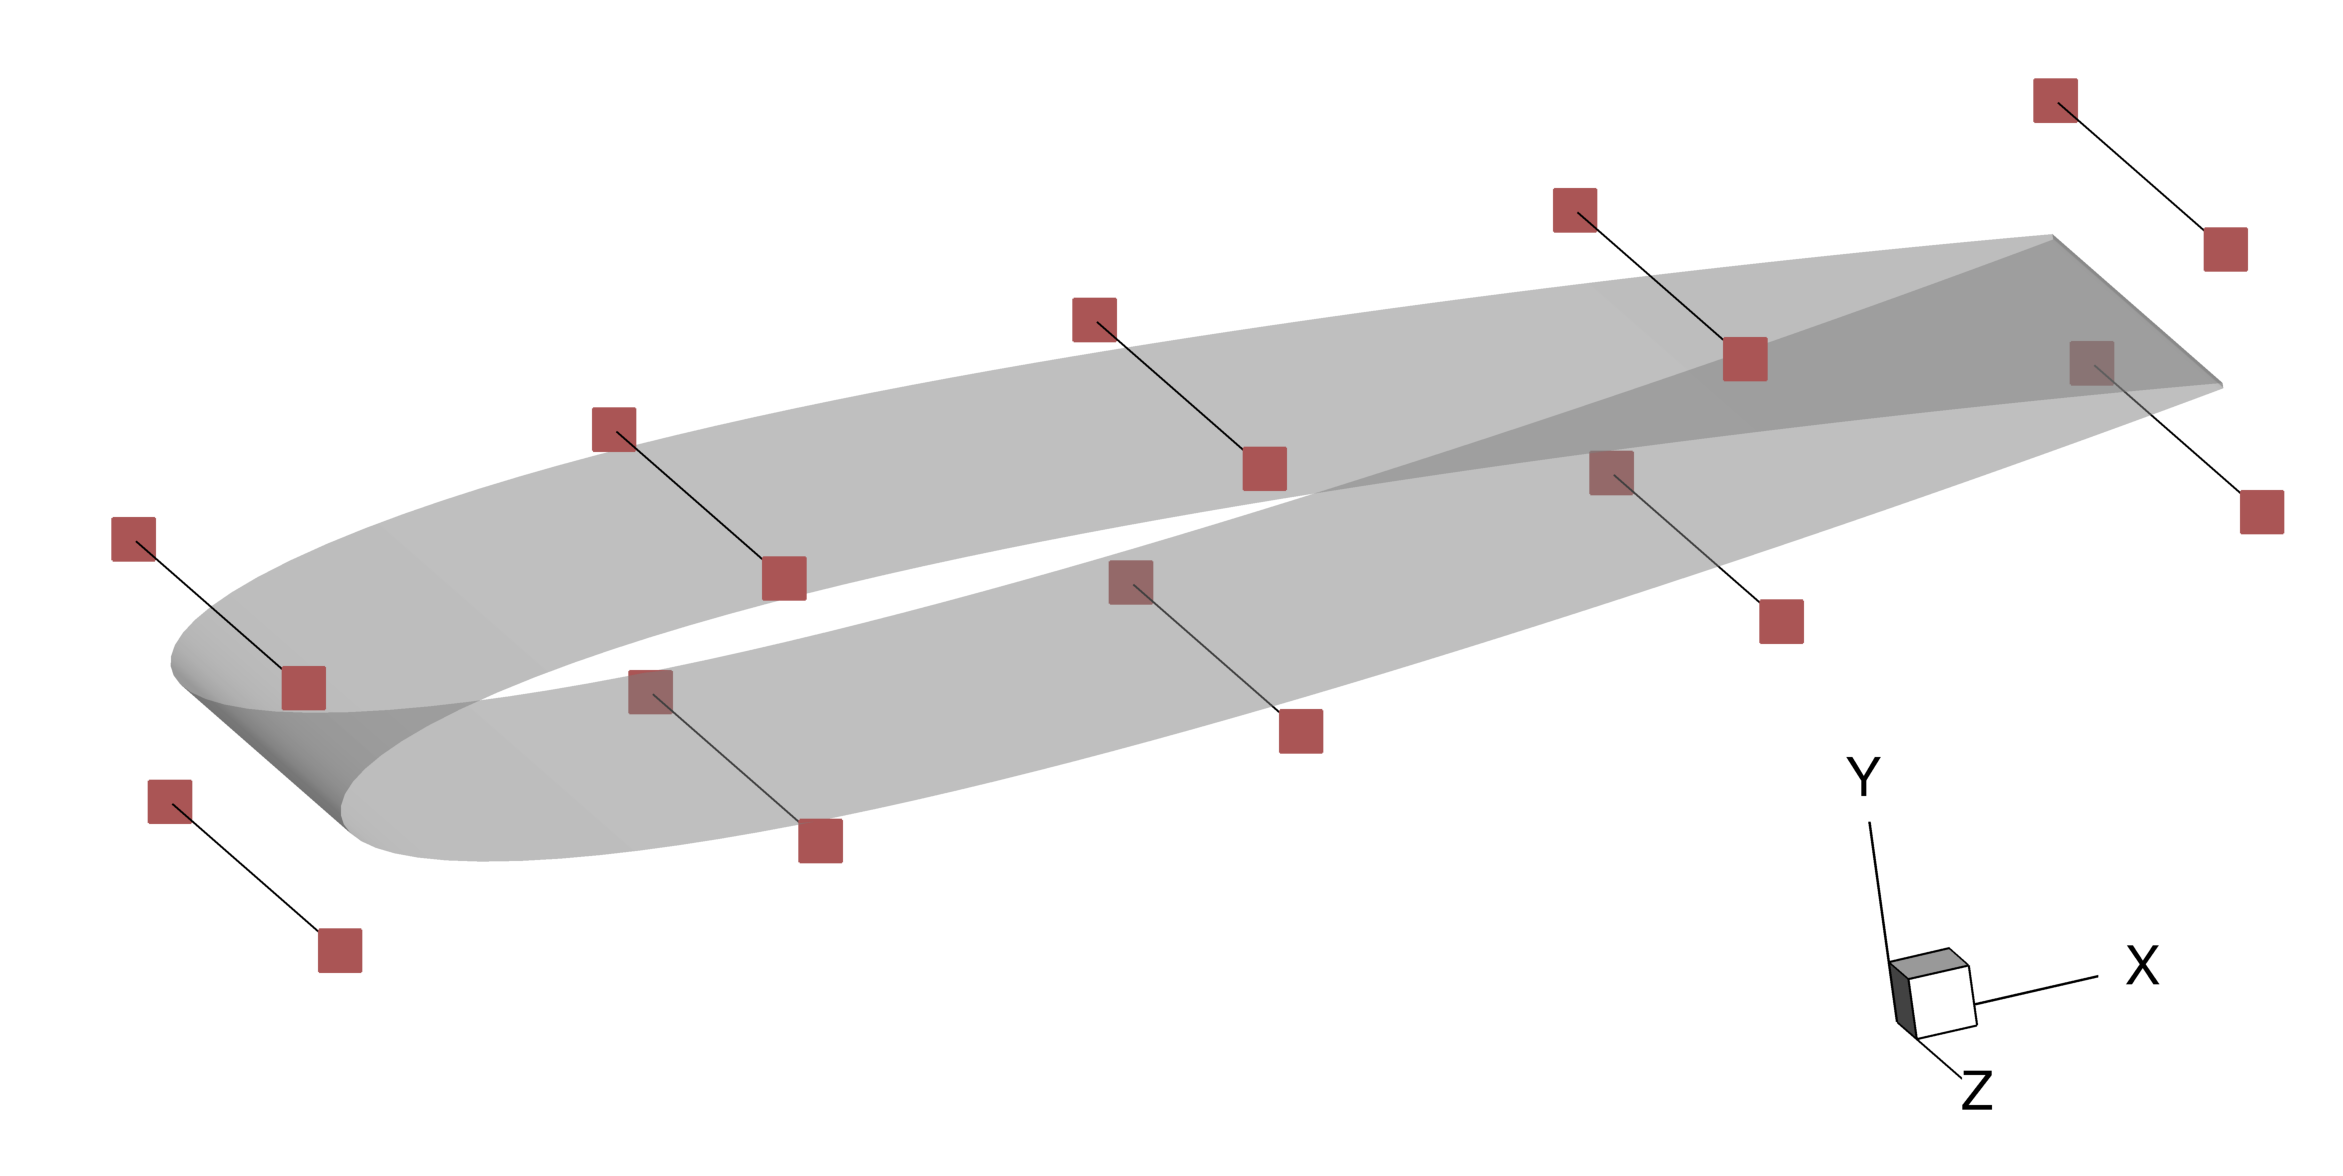
\includegraphics[width=0.8\linewidth]{images/linearConst1.png} 
  \caption{Black lines linking the FFD points movement between k=0 and k=1.}
\end{figure}

\end{frame}
%---------------------------------------------------------------%

%---------------------------------------------------------------%
\begin{frame}[fragile]{The \texttt{runScript.py} script (10/11)}

  \scriptsize
  \lstset{ language=python }
  \begin{lstlisting}
# Create a linear constraint to fix the leading and trailing point.
indSetA = []
indSetB = []
for i in [0, nFFDs_x - 1]:
    # do not constrain k=1; it has been linked in the above symmetry constraint
    for k in [0]:  
        indSetA.append(pts[i, 0, k])
        indSetB.append(pts[i, 1, k])
DVCon.addLinearConstraintsShape(indSetA, indSetB, factorA=1.0, factorB=1.0, lower=0.0, upper=0.0)
# write constraint visualization to a Tecplot file
DVCon.writeTecplot("DVConstraints.dat")
\end{lstlisting}
\vspace{-0.2in}
\begin{figure}
  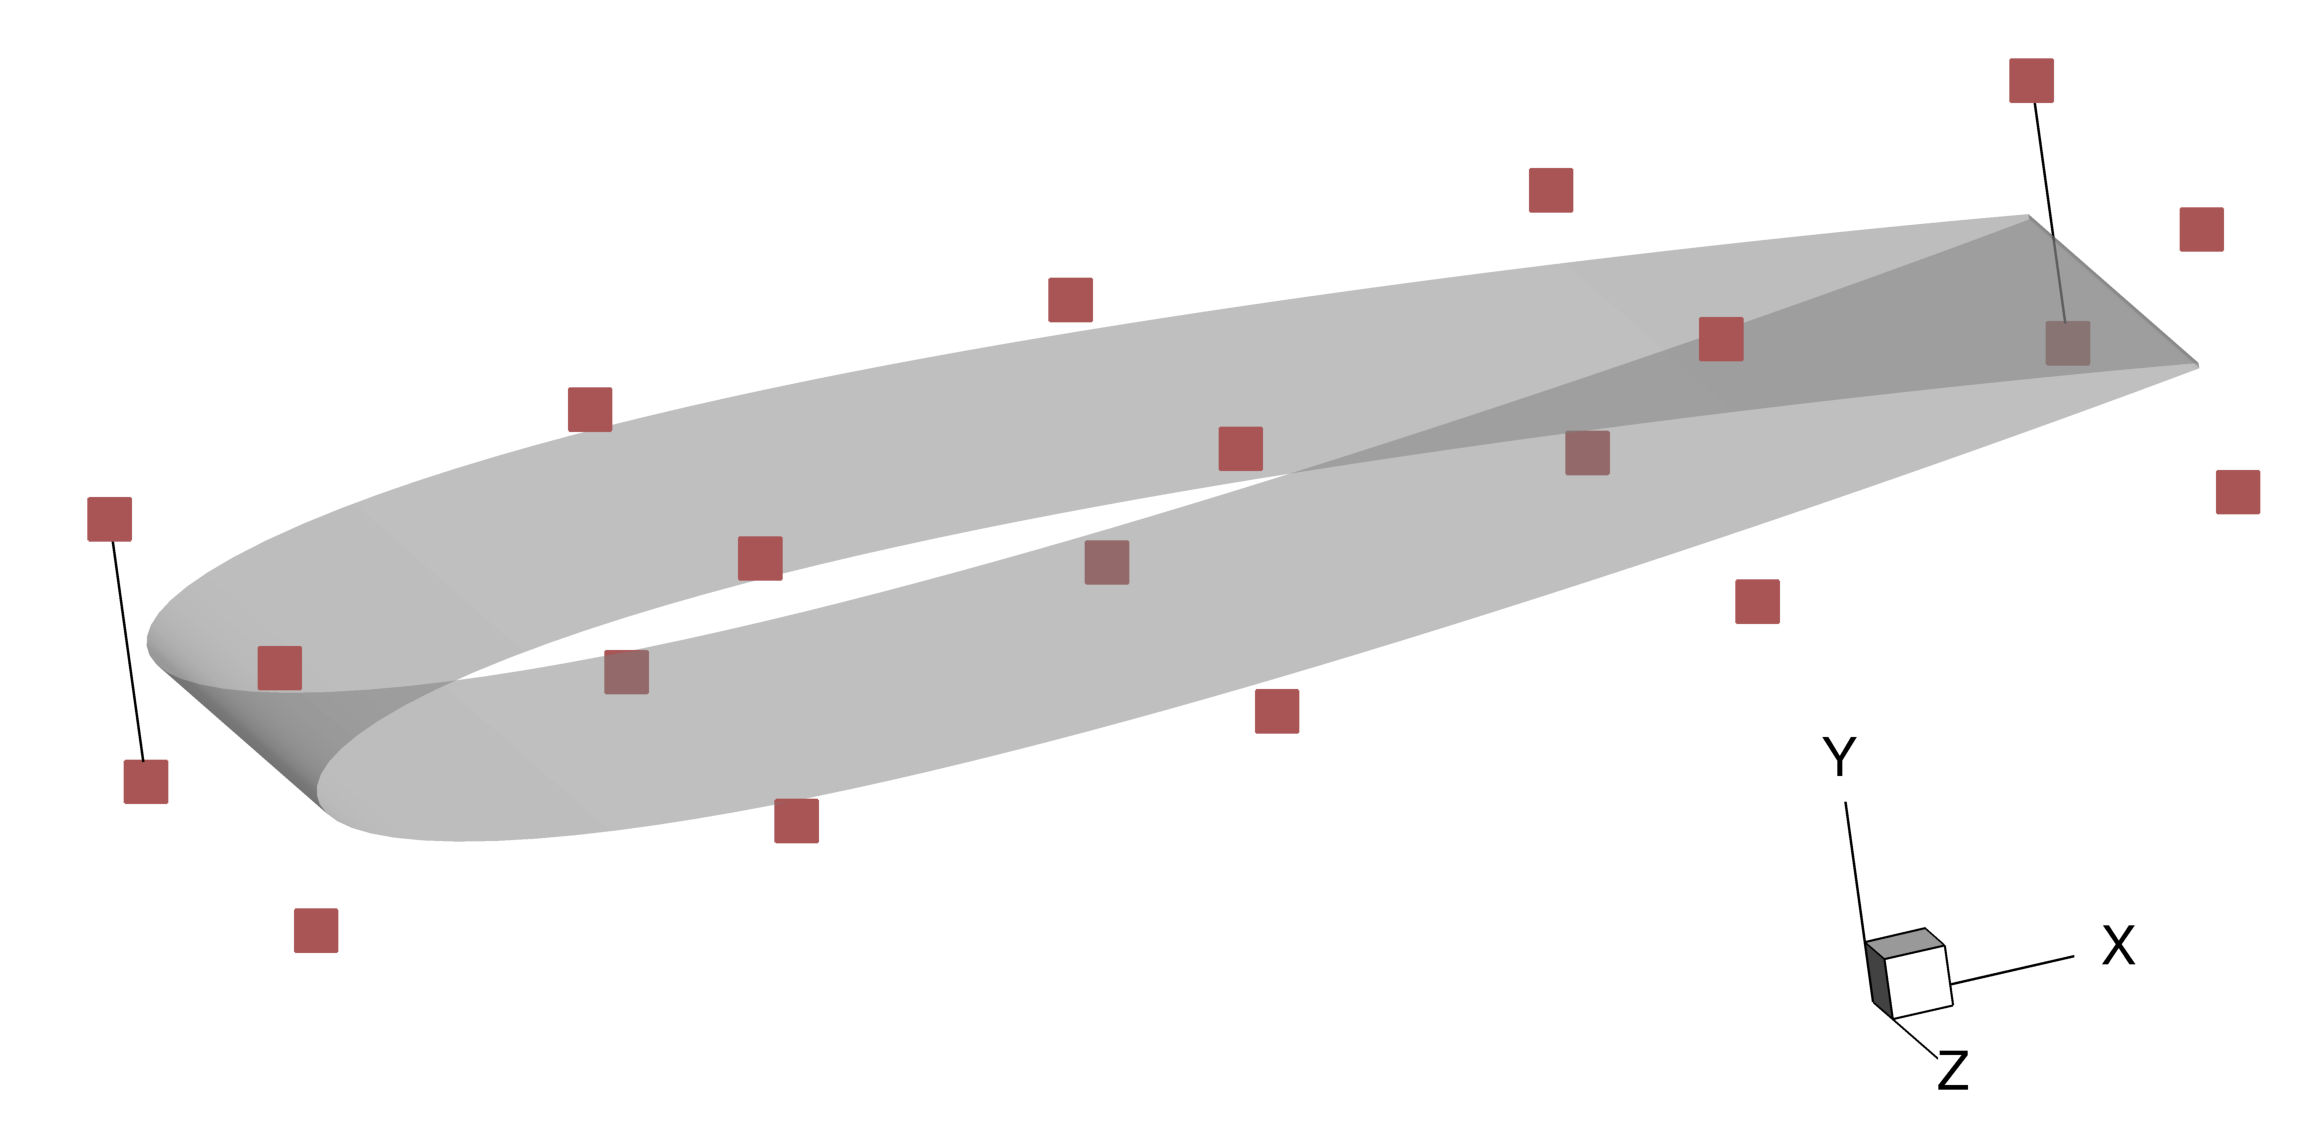
\includegraphics[width=0.8\linewidth]{images/linearConst2.png} 
  \caption{Black lines forcing the FFD points oppsitite movement at the LE and TE.}
\end{figure}

\end{frame}
%---------------------------------------------------------------%

%---------------------------------------------------------------%
\begin{frame}[fragile]{The \texttt{runScript.py} script (11/11)}

  \scriptsize
  \lstset{ language=python }
  \begin{lstlisting}
# =====================================
# Initialize optFuncs for optimization
# =====================================
optFuncs.DASolver = DASolver  # optFuncs.py has functions to run primal and adjoint
optFuncs.DVGeo = DVGeo
... # users usually don't need to change this part
# =======
# Task
# =======
if args.task == "opt":
    # run solveCL before opt. Need to specify which variables are AOA and lift
    alpha4CLTarget = optFuncs.solveCL(CL_target, "alpha", "CL")
    alpha([alpha4CLTarget], None)  # once solveCL is done, set the correct alpha
    # create an pyOptSparse opt problem and set objFun function to run primal
    optProb = Optimization("opt", objFun=optFuncs.calcObjFuncValues, comm=gcomm)
    DVGeo.addVariablesPyOpt(optProb)
    DVCon.addConstraintsPyOpt(optProb)
    optProb.addObj("CD", scale=1) # set the objective function
    optProb.addCon("CL", lower=CL_target, upper=CL_target, scale=1) # CL constraint
    if gcomm.rank == 0:
        print(optProb)
    # run graph coloring before optimization
    DASolver.runColoring()
    # set sens function to run adjoint and solve the optimization problem
    opt = OPT(args.opt, options=optOptions)
    histFile = "./%s_hist.hst" % args.opt
    sol = opt(optProb, sens=optFuncs.calcObjFuncSens, storeHistory=histFile)
    if gcomm.rank == 0:
        print(sol)

\end{lstlisting}

\end{frame}
%---------------------------------------------------------------%

%---------------------------------------------------------------%
\begin{frame}[fragile]{The \texttt{dafoam/dafoam/optFuncs.py} script (1/2)}

  \scriptsize
  \lstset{ language=python }
  \begin{lstlisting}
def calcObjFuncValues(xDV):
    """Update the design surface and run the primal solver to get objective function values.
    """
    Info("\n")
    Info("+-------------------------------------+")
    Info("|   Evaluating Objective Functions %03d |" % DASolver.nSolvePrimals)
    Info("+-------------------------------------+")
    Info("Design Variables: ")
    Info(xDV)
    a = time.time()
    # Setup an empty dictionary for the evaluated function values
    funcs = {}
    # Set the current design variables in the DV object
    DVGeo.setDesignVars(xDV)
    DASolver.setDesignVars(xDV)
    # Evaluate the geometric constraints and add them to the funcs dictionary
    DVCon.evalFunctions(funcs)
    # Solve the CFD problem
    DASolver()
    # Populate the required values from the CFD problem
    DASolver.evalFunctions(funcs, evalFuncs=evalFuncs)
    b = time.time()
    # Print the current solution to the screen
    Info("Objective Functions: ")
    Info(funcs)
    Info("Flow Runtime: %g" % (b - a))
    fail = funcs["fail"]
    return funcs, fail

\end{lstlisting}

\end{frame}
%---------------------------------------------------------------%

%---------------------------------------------------------------%
\begin{frame}[fragile]{The \texttt{dafoam/dafoam/optFuncs.py} script (2/2)}

  \scriptsize
  \lstset{ language=python }
  \begin{lstlisting}
def calcObjFuncSens(xDV, funcs):
    """Run the adjoint solver and get objective function sensitivities.
    """
    Info("+---------------------------------+")
    Info("|Evaluating Objective Function Sensitivities %03d|"%DASolver..)
    Info("+---------------------------------+")
    a = time.time()
    # write the design variable values to file
    DASolver.writeDesignVariable("designVariableHist.txt", xDV)
    # write the deform FFDs
    DASolver.writeDeformedFFDs()
    # Setup an empty dictionary for the evaluated derivative values
    funcsSens = {}
    # Evaluate the geometric constraint derivatives
    DVCon.evalFunctionsSens(funcsSens)
    # Solve the adjoint
    DASolver.solveAdjoint()
    # Evaluate the CFD derivatives
    DASolver.evalFunctionsSens(funcsSens, evalFuncs=evalFuncs)
    b = time.time()
    # Print the current solution to the screen
    with np.printoptions(precision=16, threshold=5, suppress=True):
        Info("Objective Function Sensitivity: ")
        Info(funcsSens)
        Info("Adjoint Runtime: %g s" % (b - a))
    # write the sensitivity values to file
    DASolver.writeTotalDeriv("totalDerivHist.txt", funcsSens, evalFuncs)
    fail = funcsSens["fail"]
    return funcsSens, fail
\end{lstlisting}

\end{frame}
%---------------------------------------------------------------%


%---------------------------------------------------------------%
\begin{frame}{}
  \center \Large How to change the configuration files for a new case
\end{frame}
%---------------------------------------------------------------%

%---------------------------------------------------------------%
\begin{frame}[fragile]{How to change flow conditions?}

  Change these in \texttt{runScript.py}
  \small
  \lstset{ language=python }
  \begin{lstlisting}
  U0 = 10.0
  p0 = 0.0
  nuTilda0 = 4.5e-5
  k0 = 0.015
  epsilon0 = 0.14
  omega0 = 100.0
 \end{lstlisting}

\end{frame}
%---------------------------------------------------------------%

%---------------------------------------------------------------%
\begin{frame}[fragile]{How to use more mesh cells?}

  Change the input parameters in \texttt{genAirFoilMesh.py}, e.g., reduce dX1PS, dX2PS, dXMaxPS, etc, and increase NpTE, NpExtrude.
  \footnotesize
  \lstset{ language=bash }
  \begin{lstlisting}
  ########## user input ################
  prefix = "./profiles/"
  airfoilProfilePS = prefix + "NACA0012PS.profile"
  airfoilProfileSS = prefix + "NACA0012SS.profile"
  ZSpan = 0.1  # width in the z direction
  nSpan = 2  # how many points in z
  # PS parameters
  dX1PS = 0.005  # first dx from the LE
  Alpha1PS = 1.2  # clustering from the LE
  dX2PS = 2e-3  # first dx from the TE
  Alpha2PS = 1.2  # clustering from the TE
  dXMaxPS = 0.02  # max dx for PS
  ...
  # TE parameters
  NpTE = 5  # number of points for blunt TE
  # 3D
  NpExtrude = 33  # how many points to extrude for the 3D volume mesh
  yWall = 4e-3  # first layer mesh length
  marchDist = 20.0  # march distance for extruding
  \end{lstlisting}

\end{frame}
%---------------------------------------------------------------%

%---------------------------------------------------------------%
\begin{frame}[fragile]{How to use a different turbulence model?}

  To use the kOmegaSST model, in the \texttt{constant/turbulenceProperties} file, change
  \small
  \begin{lstlisting}
  simulationType RAS;
  RAS 
  { 
      RASModel       SpalartAllmaras;  
      turbulence     on;
      printCoeffs    off;
  } 
  \end{lstlisting}

  \normalsize
  to: 

  \begin{lstlisting}
    simulationType RAS;  
    RAS 
    { 
        RASModel       kOmegaSST;  
        turbulence     on;
        printCoeffs    off;
    } 
    \end{lstlisting}


\end{frame}
%---------------------------------------------------------------%


%---------------------------------------------------------------%
\begin{frame}[fragile]{How to use more FFD points?}

  To use 40 FFD points, in the \texttt{FFD/genFFD.py} file, change
  \small
  \begin{lstlisting}
nx = [5]
ny = [2]
nz = [2]
  \end{lstlisting}

  \normalsize
  to: 

  \begin{lstlisting}
nx = [10]
ny = [2]
nz = [2]
  \end{lstlisting}

  \normalsize
  NOTE: Always use 2 points in the vertical direction, so ny=2. In addition, because in the z direction (spanwise), the airfoil is symmetry, so nz=2. For 3D wing cases, nz should be greater than 2.

\end{frame}
%---------------------------------------------------------------%


%---------------------------------------------------------------%
\begin{frame}[fragile]{How to optimize a different airfoil?}

\begin{itemize}
  \setlength\itemsep{1em}
 \item Generate the separated  upper and lower airfoil coordinates and save them to the \texttt{profiles} folder (e.g., RAE2822PS.profile and RAE2822SS.profile). Remember to delete the last few points to get blunt TE.
 \item Modify \texttt{airfoilProfilePS} and \texttt{airfoilProfileSS} in \texttt{genAirFoilMesh} to let it link to the correct airfoil coordinate files.
 \item Modify the FFD corners coordinates, i.e., \texttt{corners[0,0,:]}, \texttt{corners[0,1,:]}, etc. in the \texttt{FFD/genFFD.py} file to make sure the FFD points fully contain the new airfoil surface.
 \item Run \texttt{./Allclean.sh} to clean up the previous runs
 \item Start a Docker container and run: \\ \texttt{./preProcessing.sh \&\& python runScript.py}
\end{itemize}

\end{frame}
%---------------------------------------------------------------%

%---------------------------------------------------------------%
\begin{frame}[fragile]{How to use a different solver (1/2)?}

Refer to \texttt{examples/naca0012/subsonic}, differences in runScript.py:

  \begin{itemize}
    \setlength\itemsep{0.5em}
   \item There are new variables (e.g., T) in the global parameters. Also, we use absolute pressure p0=101325, instead of relative one
   \item "solverName" changed to "DARhoSimpleFoam"
   \item A new key "primalVarBounds" that sets the bounds for robust flow simulation
   \item In "normalizeStates", "p" is normalized by p0, insteady of dynamic pressure.
  \end{itemize}
  In addition, in the "0" folder, we have more variables, i.e., alphat and T. In the "constant" folder, the fluid properties are defined in "thermophysicalProperties" instead of "transportProperties". Also, in the "system" folder, "fvSchemes" and "fvSolution" have different setup that are specially designed for compressible flow solver DARhoSimpleFoam.
\end{frame}
%---------------------------------------------------------------%

%---------------------------------------------------------------%
\begin{frame}[fragile]{How to use a different solver (2/2)?}

  Refer to \texttt{examples/naca0012/transonic}, it is similar to \texttt{examples/naca0012/subosnic}, except that:
  
    \begin{itemize}
      \setlength\itemsep{0.5em}
     \item U0 is set to be at transonic speed
     \item "solverName" changed to "DARhoSimpleCFoam". Here C means SIMPLEC algorithm (consistent). This is needed for transonic conditions.
     \item "transonicPCOption" in "daOptions" is set to 1. This uses the transonic preconditioner to speed up the adjoint convergence
     \item In the "system" folder, "fvSchemes" and "fvSolution" have different setup that are specially designed for transonic flow conditions for DARhoSimpleCFoam.
    \end{itemize}

\end{frame}
%---------------------------------------------------------------%

%---------------------------------------------------------------%
\begin{frame}[fragile]{How to use more CPU cores?}

  If you want to run an DAFoam optimization using 4 CPU core, use this command:

  \begin{lstlisting}
  mpirun -np 4 python runScript.py | tee 2>&1 logOpt.txt
  \end{lstlisting}

  \textbf{NOTE:} Always run \texttt{./Allclean.sh} before running a new job!

\end{frame}
%---------------------------------------------------------------%

\section{Wing aerodynamic optimization}
\renewcommand{\arraystretch}{2}

%---------------------------------------------------------------%
\begin{frame}{}
  \center \Large Wing aerodynamic optimization
\end{frame}
%---------------------------------------------------------------%

%---------------------------------------------------------------%
\begin{frame}[fragile]{Optimization summary}
  \begin{table}
    \renewcommand{\arraystretch}{1.5}
    \small
    \centering
    \begin{tabular}{llllllllllll}
    \hline
    Optimizer   & IPOPT \\
    Flow and adjoint solvers  & DARhoSimpleFoam  \\
    Geometry  & Onera\_M6 \\
    Mesh  & 7\,800 cells\\
    Objective function  & $C_d$ \\
    Design variables & 120 FFDs and $\alpha$ \\
    Constraint & $C_l=0.25$, thickness, volume, TE/LE \\
    $U_\infty$  & 100 m/s \\
    $Re$  & 5$\times10^6$\\
    Turbulence Model  & Spalart--Allmaras\\
     \hline
    \end{tabular}
  \end{table}
\end{frame}
%---------------------------------------------------------------%

%---------------------------------------------------------------%
\begin{frame}[fragile]{Mesh and FFD}
  \begin{figure}
    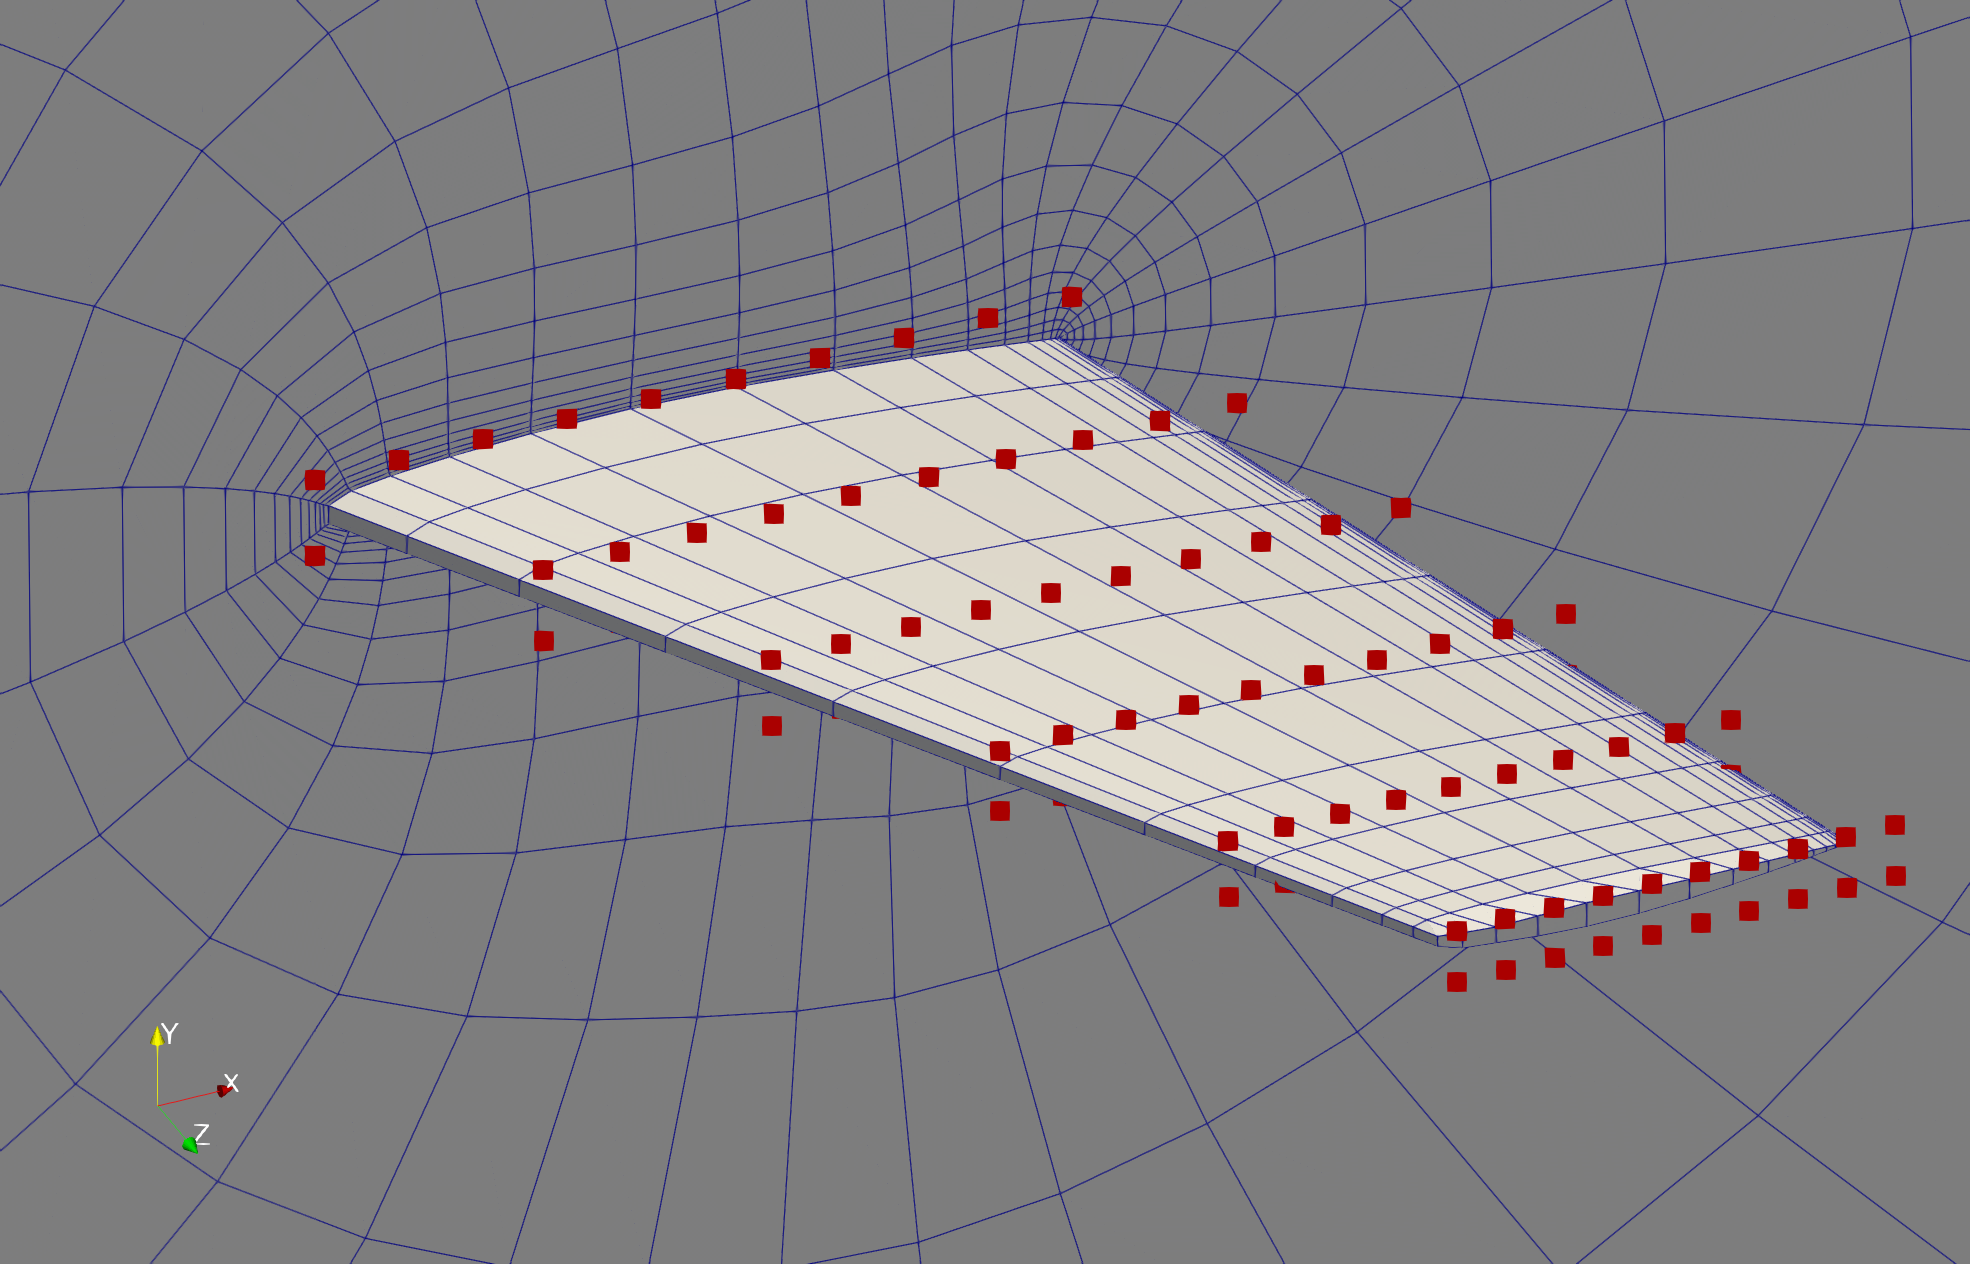
\includegraphics[width=\linewidth]{images/M6_FFD.png} 
  \end{figure}
\end{frame}
%---------------------------------------------------------------%


%---------------------------------------------------------------%
\begin{frame}[fragile]{How to run a wing optimization}

  Running a 3D wing optimization is similar to running an airfoil optimization. Open a new Docker container, and run this command for pre-processing (mesh generation):
  \footnotesize
  \lstset{ language=bash }
  \begin{lstlisting}
  ./preProcessing.sh
  \end{lstlisting}
  \normalsize

  Then, use this command to run the flow simulation: 
  \footnotesize
  \lstset{ language=bash }
  \begin{lstlisting}
  python runScript.py | tee 2>&1 logOpt.txt
  \end{lstlisting}
  \normalsize

  The optimization log will be printed to the screen and saved to \texttt{logOpt.txt}. In addition, the optimizer will write a separate log to the disk. For the IPOPT optimizer we use in this tutorial, it is \texttt{opt\_IPOPT.txt}.

\end{frame}
%---------------------------------------------------------------%

%---------------------------------------------------------------%
\begin{frame}[fragile]{The \texttt{preProcessing.sh} script}

  The overall mesh generation process is similar to the airfoil case. The main differene is that: 

  \begin{itemize}
  \item We need to provide a surface mesh in the cgns or plot3D format (e.g., surfaceMesh.cgns). The surface mesh is usually generated by using commercial software such as ICEM-CFD and Pointwise. Refer to the MACH-Aero documentation for more details. \url{https://mdolab-mach-aero.readthedocs-hosted.com/en/latest/machAeroTutorials/overset_surface_mesh.html}
  \item We coarsen the surface mesh four times to create a very coarse volume mesh for demonstration. If you want to increase the mesh density, comment out one or more these lines: \texttt{cgns\_utils coarsen surfaceMesh.cgns}
  \item The genWingMesh.py is used to extrude the surface mesh to volume mesh using pyHyp
  \end{itemize}

  NOTE: We can run \texttt{preProcessing\_snappyHexMesh.sh} to generate unstructured mesh instead. Refer to this link for more details: \url{https://cfd.direct/openfoam/user-guide/v6-snappyhexmesh/}

\end{frame}
%---------------------------------------------------------------%

%---------------------------------------------------------------%
\begin{frame}[fragile]{The \texttt{runScript.py} script (1/4)}

  The \texttt{runScript.py} script is similar to the airfoil (subsonic) case. The main differene is that: 

  1. In the design variable setup, we create a reference axis (blue line) aligned with z and located at 25\% chordwise (xFraction=0.25). Here nTwists=6 is the number of FFD layers in z. This ref axis will be used to twist the wing at these 6 spanwise locations
  
  \footnotesize
  \lstset{ language=bash }
  \begin{lstlisting}
  nTwists = DVGeo.addRefAxis("bodyAxis", xFraction=0.25, alignIndex="k")
  \end{lstlisting}
  \vspace{-0.15in}
  \begin{figure}
    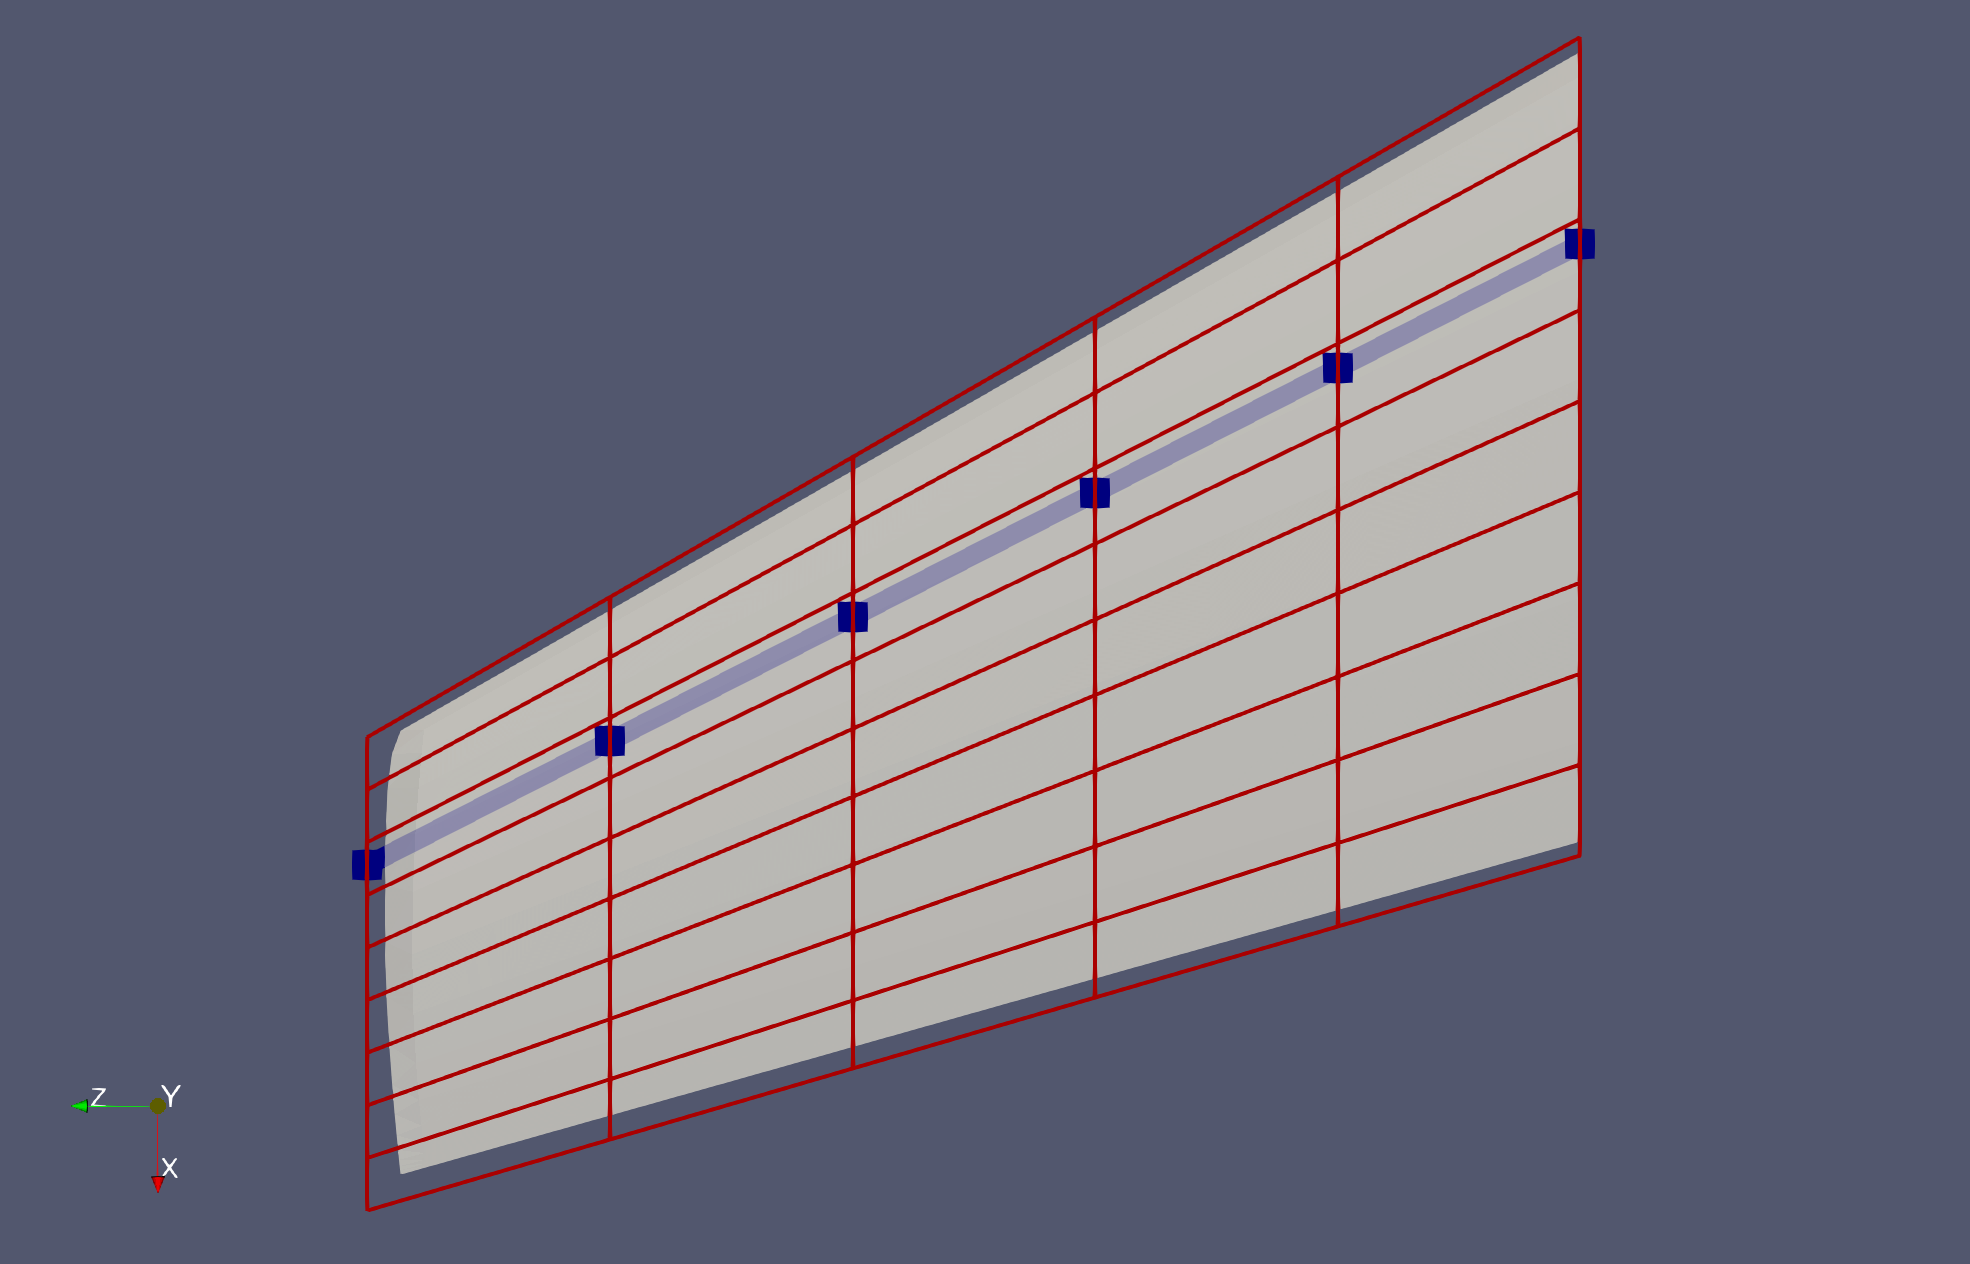
\includegraphics[width=0.65\linewidth]{images/M6_RefAxis.png} 
  \end{figure}

\end{frame}
%---------------------------------------------------------------%

%---------------------------------------------------------------%
\begin{frame}[fragile]{The \texttt{runScript.py} script (2/4)}

  2. Similar to the alpha(val,geo) function, we define a twist(val, geo) function to twist the wing. Here we loop over all the spanwise locations except for the root and assign the design variable values from \texttt{val} to \texttt{geo.rot\_z["bodyAxis"].coef[i]}. Then the \texttt{geo} object will actually twist the wing during optimization. Note that the first element in \texttt{val}, i.e., \texttt{val[0]} is the 2nd twist to the root, but \texttt{geo.rot\_z["bodyAxis"].coef[0]} is the root twist, that is why we use \texttt{val[i-1]}.
  
  \footnotesize
  \lstset{ language=python }
  \begin{lstlisting}
  def twist(val, geo):
      for i in range(1, nTwists):
          geo.rot_z["bodyAxis"].coef[i] = val[i - 1]
  \end{lstlisting}

  \normalsize
  After that, we add the twist as the design variable. Again, we have only nTwists-1 twist variables, and their initial values are all zeros: \texttt{np.zeros(nTwists-1)}.

  \footnotesize
  \lstset{ language=python }
  \begin{lstlisting}
  # twist
  DVGeo.addGeoDVGlobal("twist", np.zeros(nTwists - 1), twist, lower=-10.0, upper=10.0, scale=1.0)
  daOptions["designVar"]["twist"] = {"designVarType": "FFD"}
  \end{lstlisting}

\end{frame}
%---------------------------------------------------------------%

%---------------------------------------------------------------%
\begin{frame}[fragile]{The \texttt{runScript.py} script (3/4)}

  3. Similar to the airfoil case, we need to define LE (red) and TE (blue) lines for the thickness and volume constraints
  \footnotesize
  \lstset{ language=bash }
  \begin{lstlisting}
  leList = [[0.01, 0.0, 1e-3], [0.7, 0.0, 1.19]]
  teList = [[0.79, 0.0, 1e-3], [1.135, 0.0, 1.19]]
  \end{lstlisting}
  \vspace{-0.15in}
  \begin{figure}
    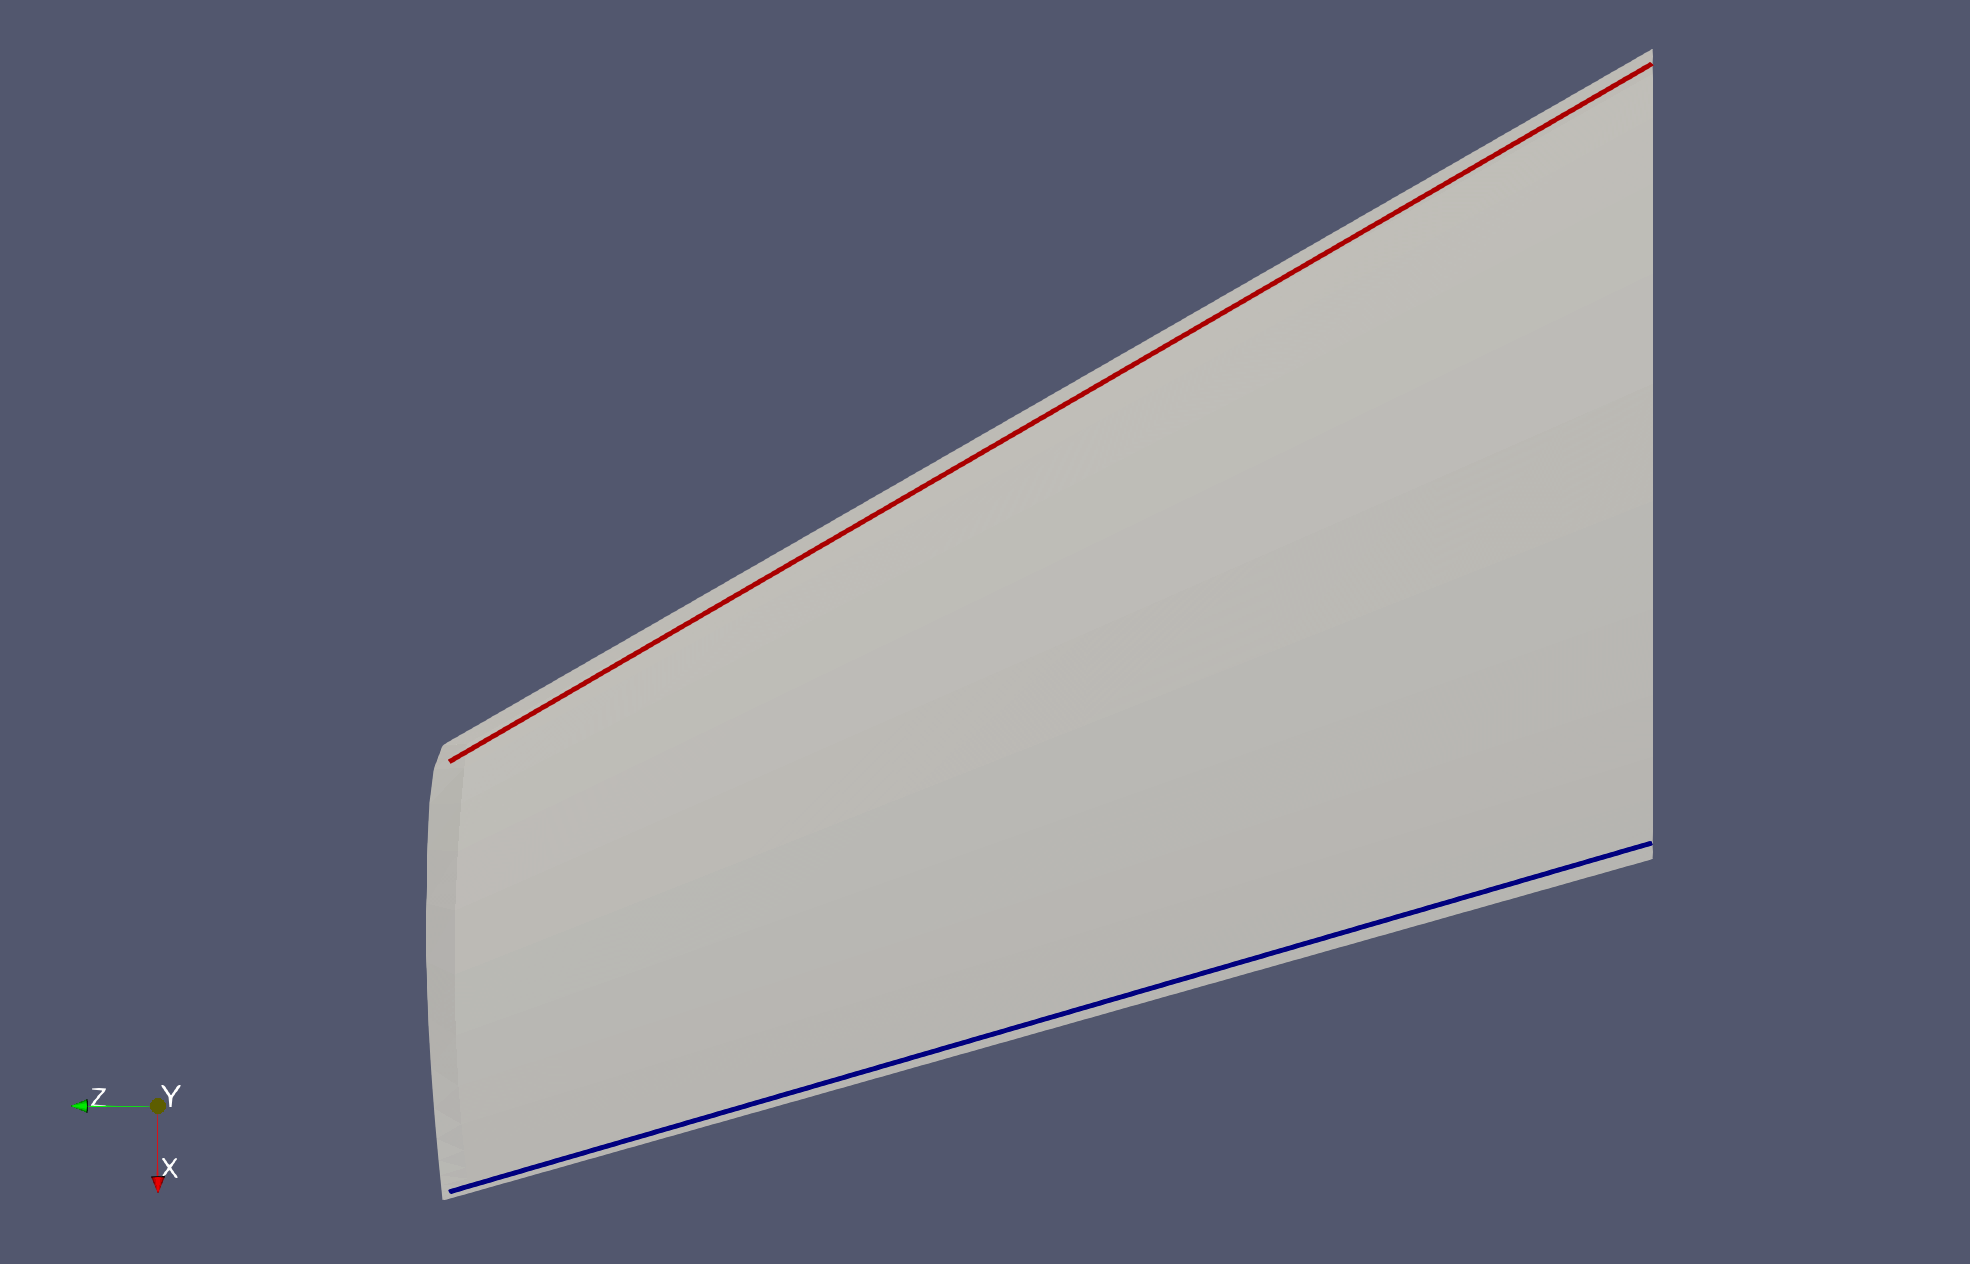
\includegraphics[width=0.6\linewidth]{images/M6_LETE.png} 
  \end{figure}
  \vspace{-0.15in}
  \normalsize
  We do not impose symmetry constraints because it is a 3D case. Also, the LE and TE constrainst can be easily added by calling:

  \footnotesize
  \lstset{ language=bash }
  \begin{lstlisting}
  DVCon.addLeTeConstraints(0, "iLow")
  DVCon.addLeTeConstraints(0, "iHigh")
  \end{lstlisting}

\end{frame}
%---------------------------------------------------------------%

%---------------------------------------------------------------%
\begin{frame}[fragile]{The \texttt{runScript.py} script (4/4)}

  4. There are other minor changes, e.g., we add a "checkMeshThreshold" parameter in "daOptions" to relax the mesh quality tolerance, in "meshOptions", we have only one symmetry plane, as opposed to two symmetry planes in the airfoil case. 
  
\end{frame}
%---------------------------------------------------------------%

%---------------------------------------------------------------%
\begin{frame}[fragile]{Useful links}

  \begin{itemize}
  \item OpenFOAM user guide: \url{https://www.openfoam.com/documentation/user-guide}
  \item DAFoam documentation: \\ \url{https://dafoam.github.io}
  \item MACH-Aero documentation: \url{https://mdolab-mach-aero.readthedocs-hosted.com}
  \end{itemize}
  
\end{frame}
%---------------------------------------------------------------%

%---------------------------------------------------------------%
\begin{frame}[plain]{}
  \Huge \centering
  Thank you!
\end{frame}
%---------------------------------------------------------------%

\end{document}
